\chapter{Μοντέλο πρόβλεψης απόδοσης απαντήσεων μέσω προτροπής}
\label{ch:chapter4}

Στο Κεφάλαιο \ref{ch:chapter3} παρουσιάστηκε η μεθοδολογία που
ακολουθήθηκε για την συλλογή των δεδομένων και την αξιολόγηση των
απαντήσεων του μοντέλου του \textlatin{GitHub Copilot}. Η
κατηγοριοποίηση των δεδομένων, οδήγησε στην ιδέα να αναπτυχθεί ένα
μοντέλο μηχανικής μάθησης με σκοπό την πρόβλεψη της απόδοσης μιας
απάντησης του μοντέλου του \textlatin{GitHub Copilot}, με βάση την
προτροπή.

Aρχικά έγινε η προσπάθεια για την πρόβλεψη της
ακριβούς τιμής της αξιολόγησης, από πολύ αρνητική έως πολύ θετική, αλλά,
λόγω του μικρού μεγέθους των δεδομένων, η παραπάνω λογική οδήγησε σε
εξαιρετικά ασυνεπή αποτέλεσματα, με ακρίβεια χαμηλότερη αυτής των
πενήντα τοις εκατό (50\%). Συνεπώς, αποφασίστηκε να γίνει η προσπάθεια
κατηγοριοποίησης της απάντησης είτε σε θετική αξιολόγηση, είτε σε
αρνητική.

\section{Κατηγοριοποίηση των δεδομένων}

Για την κατηγοριοποίηση των δεδομένων, η κάθε προτροπή επεξεργάστηκε,
προκειμένου να αφαιρεθούν τα κομμάτια κώδικα από την υπόλοιπη προτροπή
και έπειτα αφαιρέθηκαν οι "κενές λέξεις" (\textlatin{stopwords}) με την
χρήση της βιβλιοθήκης \textlatin{Natural Language Toolkit (NLTK)}. Για
κάθε προτροπή που είχε κομμάτια κώδικα, ο αριθμός των συμβόλων
(\textlatin{symbols}), αποθηκεύθηκε σε μια άλλη κατηγορία.

Ένα από τα μεγαλύτερα προβλήματα των Γλωσσικών Μοντέλων, είναι ο
μέγιστος αριθμός των συμβόλων (\textlatin{tokens}) που μπορούν να
επεξεργαστούν. Καθώς οι προτροπές ζητούσαν μεγάλα κομμάτια κώδικα, ειδικά στις
περιπτώσεις των ελέγχων του κώδικα, το μοντέλο συχνά έφτανε στο όριο των
δεδομένων που μπορούσε να παράξει στην απάντησή του. Καθώς το μοντέλο
δεν γνώριζε εκ των προτέρων το μέγεθος της απάντησης, αν ο
προγραμματιστής δεν το παρότρυνε να σταματήσει σε ένα συγκεκριμένο
αριθμό συμβόλων, το μοντέλο θα συνέχιζε να παράγει κώδικα μέχρι να
φτάσει στο όριο των δεδομένων που μπορούσε να παράξει, οδηγώντας σε μια
σειρά από αποτυγχημένες απαντήσεις.

Για την αντιμετώπιση του προβλήματος, ζητήθηκε από το
μοντέλο να απαντάει για ένα συγκεκριμένο μέρος του προβλήματος, όπως
παραδείγματος χάρη έναν συγκεκριμένο έλεγχο, αντί όλων των ελέγχων.
΄Επειτα, ζητήθηκε από το το μοντέλο να περιμένει την προτροπή με
περιεχόμενο την λέξη "\textlatin{continue}" (συνέχισε), προκειμένου να
συνεχίσει με την προηγούμενη απάντησή του. Με αυτόν τον τρόπο, το
μοντέλο θα μπορούσε να απαντήσει σε μια προτροπή, χωρίς να φτάσει στο
όριο των δεδομένων που μπορούσε να παράξει.

Ωστόσο, αυτό οδήγησε σε αρκετές προτροπές με μοναδικό περιεχόμενο την
λέξη "\textlatin{continue}", που αφενός δεν είχαν καμία σχέση με το
προηγούμενο κείμενο και αφετέρου, εφ᾽ όσον ο προγραμματιστής παρότρυνε
το μοντέλο να συνεχίσει με την απάντησή του, σήμαινε πως η τουλάχιστον
αμέσως προηγούμενη απάντηση ήταν ικανοποιητική, οδηγώντας σε μια
μεροληψία προς θετικά αποτελέσματα. Συνεπώς, αποφασίστηκε να
υπολογίζεται ο συνεχόμενος αριθμός προτροπών με περιεχόμενο την λέξη
"\textlatin{continue}", συνάμα με το θέμα της προτροπής, ώστε να
δημιουργούνται ομάδες προτροπών που στοχεύουν στο ίδιο ερώτημα, αλλά
χρειάστηκε να διασπαστούν λόγω των περιορισμών του μοντέλου.

Περιπτώσεις προτροπών που είτε ματαιώθηκαν, είτε δεν είχαν απάντηση λόγω
τεχνικών προβλημάτων, ήταν σημειωμένες εξαρχής και παραλείφθηκαν από την
ανάλυση.

\subsection{Προεπεξεργασία και Προετοιμασία Δεδομένων}

Με την χρήση των βιβλιοθηκών \textlatin{pandas} και
\textlatin{scikit-learn}, η διαδικασία προεπεξεργασίας και προετοιμασίας
των δεδομένων περιελάμβανε τα ακόλουθα στάδια:
\begin{enumerate}
  \item
    \textbf{Εισαγωγή Δεδομένων:} Τα δεδομένα εισήχθησαν από ένα
    αρχείο \textlatin{CSV}
    χρησιμοποιώντας τη βιβλιοθήκη \textlatin{pandas} για τον αποτελεσματικό
    χειρισμό τους.
  \item
    \textbf{Κωδικοποίηση Κατηγορικών Μεταβλητών:} Οι κατηγορικές
    μεταβλητές "\textlatin{subject}" (θέμα) και "\textlatin{type}" (τύπος)
    κωδικοποιήθηκαν αριθμητικά με τη χρήση του \textlatin{LabelEncoder}.

  \item
    \textbf{Μετατροπή Χρονικών Δεδομένων:} Η στήλη \textlatin{"createdAt"}
    μετατράπηκε σε αριθμητική μορφή, αντιπροσωπεύοντας τα δευτερόλεπτα από
    την εποχή \textlatin{UNIX} (1/1/1970).

  \item
    \textbf{Δυαδικοποίηση Αξιολογήσεων:} Η στήλη \textlatin{"rating"}
    (αξιολόγηση) μετατράπηκε σε δυαδική μορφή, όπου οι θετικές
    αξιολογήσεις αντιστοιχήθηκαν στην τιμή ένα (1) και οι αρνητικές στην
    τιμή μηδέν (0).

  \item
    \textbf{Ομαδοποίηση Δεδομένων:} Πραγματοποιήθηκε ομαδοποίηση των
    δεδομένων με βάση τη στήλη \textlatin{"group"}. Για κάθε ομάδα,
    υπολογίστηκαν διάφορα στατιστικά μέτρα, όπως ο μέσος όρος για τις
    αριθμητικές μεταβλητές και η επικρατούσα τιμή για τις κατηγορικές.

  \item
    \textbf{Επεξεργασία Κειμένου:} Εφαρμόστηκε η τεχνική \textlatin{Term
    Frequency-Inverse Document Frequency (TF-IDF)} για τη μετατροπή των
    κειμενικών προτροπών σε αριθμητικά χαρακτηριστικά. Η στήλη
    \textlatin{"prompt"} (προτροπή) μετασχηματίστηκε σε πολλαπλές στήλες,
    κάθε μία εκ των οποίων αντιπροσωπεύει ένα διακριτό χαρακτηριστικό
    \textlatin{TF-IDF}.

  \item
    \textbf{Διαχείριση Ελλιπών Τιμών:} Οι ελλιπείς τιμές στις αριθμητικές
    στήλες αντικαταστάθηκαν με τη μέση τιμή της αντίστοιχης στήλης,
    διασφαλίζοντας την πληρότητα του συνόλου δεδομένων.
\end{enumerate}

\subsection{Επιλογή Χαρακτηριστικών}

Η διαδικασία επιλογής χαρακτηριστικών περιελάμβανε τα εξής βήματα:
\begin{enumerate}
  \item
    \textbf{Εφαρμογή \textlatin{SelectKBest}:} Χρησιμοποιήθηκε η μέθοδος
    \textlatin{SelectKBest} σε συνδυασμό με τη συνάρτηση (${\chi}^2$) για
    την επιλογή των δέκα (10) πιο σημαντικών χαρακτηριστικών. Αυτή η
    προσέγγιση συνέβαλε στη μείωση της διαστατικότητας του προβλήματος και
    στην επικέντρωση στα πλέον πληροφοριακά χαρακτηριστικά.

  \item
    \textbf{Διαχωρισμός Δεδομένων:} Τα δεδομένα διαχωρίστηκαν σε σύνολα
    εκπαίδευσης και ελέγχου, με αναλογία ογδόντα τοις εκατό (80\%) και
    είκοσι τοις εκατό (20\%) αντίστοιχα, χρησιμοποιώντας τη συνάρτηση
    \textlatin{train\_test\_split}.
\end{enumerate}

\section{Εκπαίδευση και Αξιολόγηση Μοντέλων}

Για την εκπαίδευση και αξιολόγηση των μοντέλων ακολουθήθηκε η εξής
διαδικασία:
\begin{enumerate}
  \item
    \textbf{Επιλογή Αλγορίθμων:} Επιλέχθηκαν πέντε διαφορετικοί
    αλγόριθμοι μηχανικής μάθησης: \tl{Random Forest, Support Vector
    Machine (SVM), Gradient Boosting, MetaCost} και \tl{Naive Bayes}.
  \item
    \textbf{Βελτιστοποίηση Υπερπαραμέτρων:} Για κάθε αλγόριθμο,
    πραγματοποιήθηκε εκτενής αναζήτηση πλέγματος (\tl{Grid Search}) με
    δεκάπτυχη διασταυρωμένη επικύρωση για τη βελτιστοποίηση των
    υπερπαραμέτρων.
  \item
    \textbf{Εκπαίδευση Μοντέλων:} Τα μοντέλα εκπαιδεύτηκαν χρησιμοποιώντας
    τις βέλτιστες υπερπαραμέτρους που προέκυψαν από την αναζήτηση
    πλέγματος.
  \item
    \textbf{Αξιολόγηση Μοντέλων:} Η απόδοση των μοντέλων αξιολογήθηκε
    χρησιμοποιώντας το σύνολο ελέγχου. Υπολογίστηκαν μετρικές όπως η
    ακρίβεια, η ανάκληση και το \tl{F1-score}.
  \item
    \textbf{Οπτικοποίηση Αποτελεσμάτων:} Δημιουργήθηκαν πίνακες σύγχυσης
    (\tl{confusion matrices}) και συγκριτικά γραφήματα για την οπτική
    αναπαράσταση της απόδοσης των διαφόρων μοντέλων.
\end{enumerate}

Η μεθοδολογία αυτή επέτρεψε τη συστηματική ανάπτυξη, εκπαίδευση και
αξιολόγηση των μοντέλων, παρέχοντας μια ολοκληρωμένη εικόνα της απόδοσής
τους στην ταξινόμηση των δεδομένων.

Πραγματοποιήθηκε επίσης έρευνα για την επιλογή ανάπτυξης ενός νευρωνικού
δικτύου, αλλά λόγω του μικρού μεγέθους των δεδομένων, το αποτέλεσμα ήταν
ανεπαρκή, με ακρίβεια κάτω του πενήντα τοις εκατό (50\%). Με την
εφαρμογή των παραπάνω βημάτων, η ακρίβεια των μοντέλων αυξήθηκε
σημαντικά, με τα αποτελέσματα να αναλύονται παρακάτω.

\begin{figure}[H]
  \begin{center}
    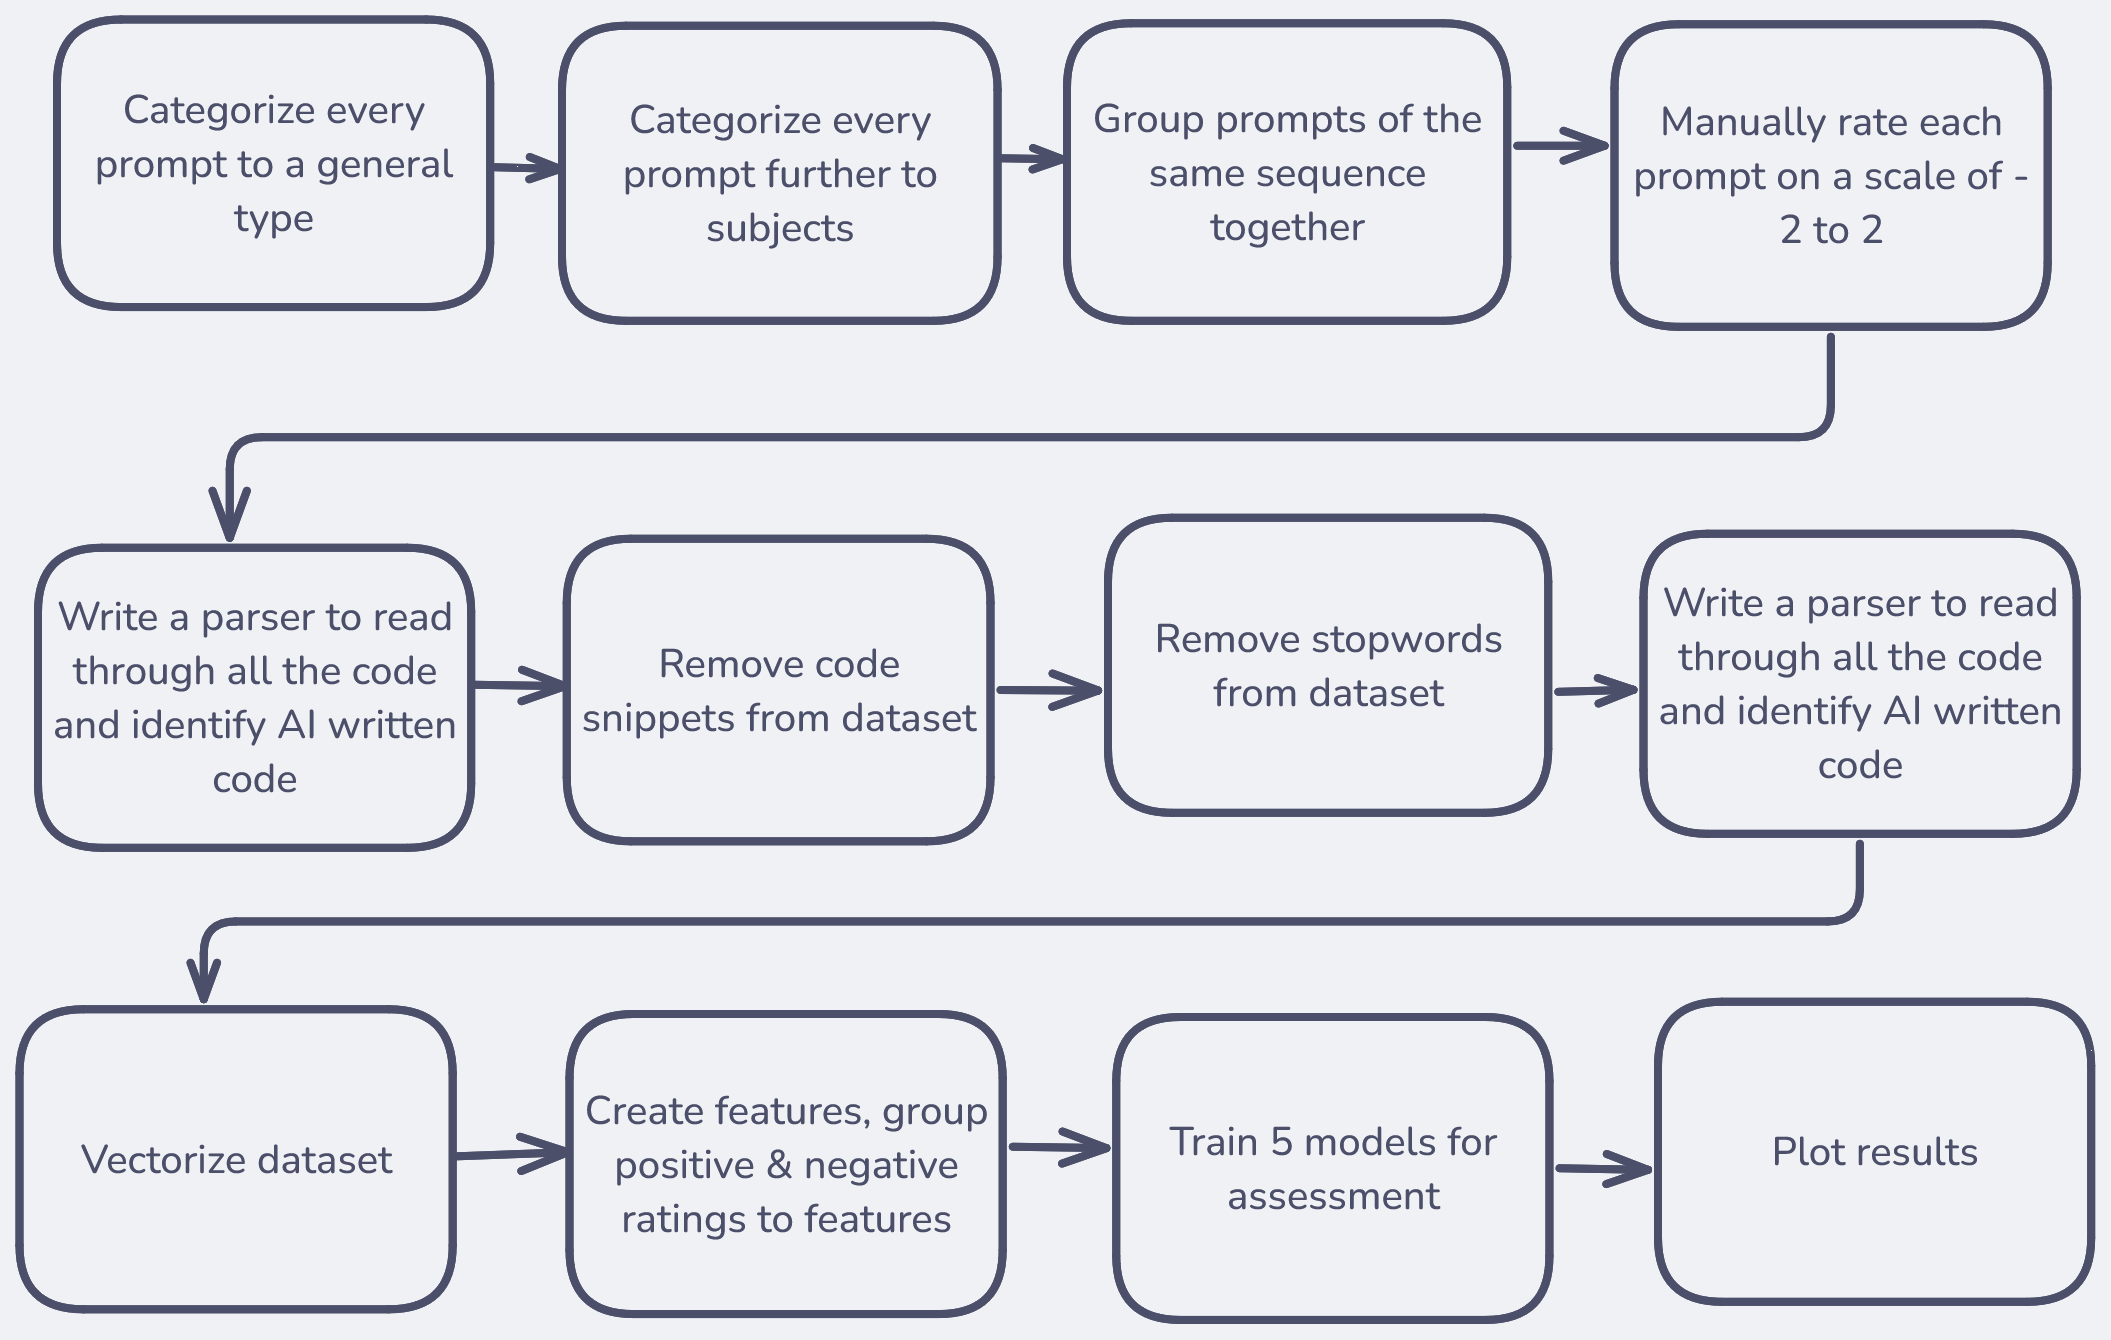
\includegraphics[width=0.9\textwidth]{excalidraw2.png}
    \caption{Διάγραμμα Ανάπτυξης Μοντέλου}
  \end{center}
  \label{fig:excalidraw2}
\end{figure}

\section{Αποτελέσματα}

Η ανάπτυξη ενός μοντέλου πρόβλεψης της απόδοσης Γλωσσικών Μοντέλων μέσω
πολλαπλών κριτηρίων, με ιδιαίτερη έμφαση στην προτροπή, αποτελεί ένα
καινοτόμο ερευνητικό εγχείρημα. Ο όρος "μηχανική προτροπής"
(\textlatin{Prompt Engineering}) αναφέρεται στη εξειδικευμένη
μεθοδολογία σχεδιασμού και βελτιστοποίησης προτροπών με στόχο τη
μεγιστοποίηση της απόδοσης του μοντέλου \cite{10.1162/tacl_a_00324,
chen2024unleashingpotentialpromptengineering}.

Οι επιστημονικές έρευνες στον ραγδαία εξελισσόμενο τομέα αυτό είναι
ιδιαίτερα πρόσφατες, με την πλειονότητα των σημαντικών δημοσιεύσεων να
εμφανίζεται μετά τη δημόσια κυκλοφορία του \textlatin{ChatGPT}
\cite{greshake2023youvesignedforcompromising,
white2023promptpatterncatalogenhance}. Ωστόσο, η αποτελεσματική
εφαρμογή και βελτιστοποίηση της μηχανικής προτροπής αποτελεί ένα από τα
πιο κρίσιμα και πολύπλοκα προβλήματα ενός κόσμου ολοένα και περισσότερο
ενισχυμένου από την τεχνητή νοημοσύνη.

Η εξαγωγή του μέγιστου δυνατού επιπέδου απόδοσης από τα Γλωσσικά
Μοντέλα και κατ' επέκταση η μείωση σφαλμάτων και μη ικανοποιητικών
αποκρίσεων, με σκοπό την αύξηση της απόδοσης χωρίς
την εισαγωγή επιπρόσθετων δεδομένων ή την τροποποίηση του υπάρχοντος
κώδικα ανάπτυξης του μοντέλου, αποτελεί μια διαδικασία τόσο δύσκολη όσο
και δυσνόητη. Η αξιοποίηση ενός μοντέλου μηχανικής μάθησης για την
πρόβλεψη της απόδοσης ενός γλωσσικού μοντέλου μέσω της προτροπής
δύναται να παράσχει πολύτιμα εργαλεία για τη μεγιστοποίηση της απόδοσης.

\begin{figure}[H]
  \begin{center}
    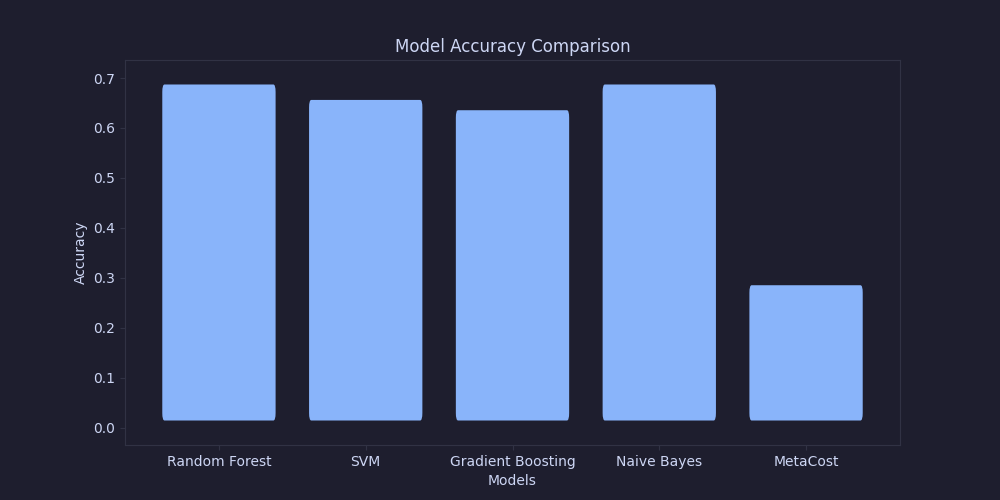
\includegraphics[width=0.9\textwidth]{model_accuracy_comparison.png}
    \caption{Σύγκριση ακρίβειας μοντέλων}
  \end{center}
  \label{fig:accuracy}
\end{figure}

Το παραπάνω σχήμα παρουσιάζει την ακρίβεια των μοντέλων που
αναπτύχθηκαν. Συγκεκριμένα:

\begin{enumerate}
  \item \tl{Random Forest} (Ακρίβεια: 70,10\%):
  \item \tl{SVM} (Ακρίβεια: 67,01\%):
  \item \tl{Gradient Boosting} (Ακρίβεια: 68,04\%):
  \item \tl{Naive Bayes} (Ακρίβεια: 70,10\%):
  \item \tl{MetaCost} (Ακρίβεια: 29.89\%)
\end{enumerate}

Το μοντέλο \tl{Random Forest} μαζί με το \tl{Naive Bayes}
αποδείχθηκαν τα πιο αποτελεσματικά μοντέλα στην πρόβλεψη των
απαντήσεων, με το μοντέλο \tl{MetaCost} να έχει την χειρότερη απόδοση
με διαφορά. Για μια πιο στοχευμένη ανάλυση των αποτελεσμάτων,
παρατίθενται οι πίνακες σύγχυσης των μοντέλων και διαγράμματα σύγκρισης των αποδόσεων των μοντέλων ανά τύπο και θέμα προτροπής:

\begin{figure}[H]
  \begin{center}
    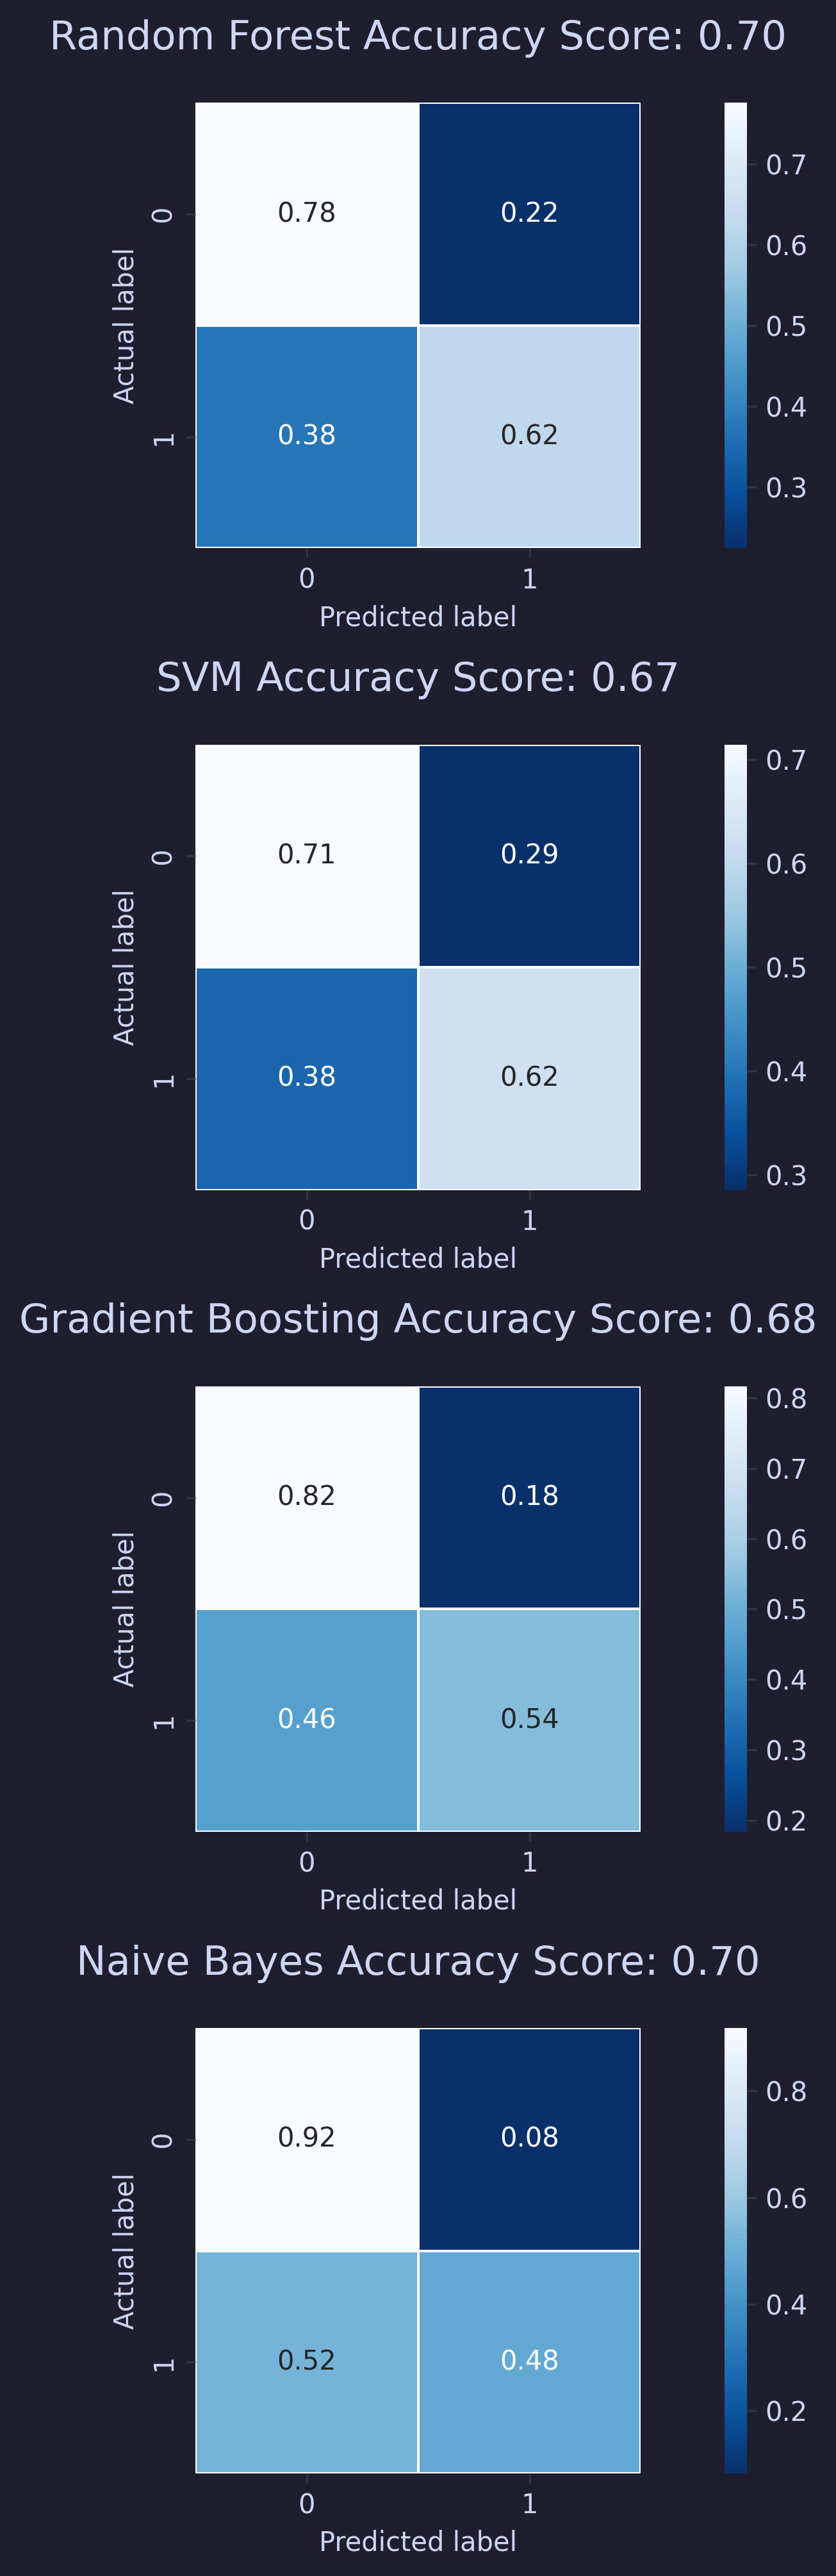
\includegraphics[height=0.85\textheight]{confusion_matrix.png}
    \caption{Πίνακες Σύγχυσης μοντέλων}
  \end{center}
  \label{fig:confusionmatrix}
\end{figure}

Για κάθε αλγόριθμο, ο πίνακας σύγχυσης δείχνει την απόδοση στην
πρόβλεψη δύο κλάσεων, 0 και 1, αναπαραστώντας τις αρνητικές και
θετικές αξιολογήσεις αντίστοιχα.
Αναλύοντας τους πίνακες:

\begin{enumerate}
  \item \tl{Random Forest}:
    \begin{itemize}
      \item Σωστές προβλέψεις για την κλάση 0: 78\%
      \item Λανθασμένες προβλέψεις για την κλάση 0: 22\%
      \item Σωστές προβλέψεις για την κλάση 1: 62\%
      \item Λανθασμένες προβλέψεις για την κλάση 1: 38\%
    \end{itemize}

  \item \tl{SVM}:
    \begin{itemize}
      \item Σωστές προβλέψεις για την κλάση 0: 71\%
      \item Λανθασμένες προβλέψεις για την κλάση 0: 29\%
      \item Σωστές προβλέψεις για την κλάση 1: 62\%
      \item Λανθασμένες προβλέψεις για την κλάση 1: 38\%
    \end{itemize}

  \item \tl{Gradient Boosting}:
    \begin{itemize}
      \item Σωστές προβλέψεις για την κλάση 0: 82\%
      \item Λανθασμένες προβλέψεις για την κλάση 0: 18\%
      \item Σωστές προβλέψεις για την κλάση 1: 54\%
      \item Λανθασμένες προβλέψεις για την κλάση 1: 46\%
    \end{itemize}

  \item \tl{Naive Bayes}:
    \begin{itemize}
      \item Σωστές προβλέψεις για την κλάση 0: 92\%
      \item Λανθασμένες προβλέψεις για την κλάση 0: 8\%
      \item Σωστές προβλέψεις για την κλάση 1: 48\%
      \item Λανθασμένες προβλέψεις για την κλάση 1: 52\%
    \end{itemize}
\end{enumerate}

Παρατηρείται ότι ο \tl{Naive Bayes} έχει την υψηλότερη ακρίβεια στην
πρόβλεψη της κλάσης 0, αλλά τη χαμηλότερη για την κλάση 1. Ο \tl{Random
Forest} και το \tl{SVM} παρουσιάζουν πιο ισορροπημένη απόδοση μεταξύ των
δύο κλάσεων. Το \tl{Gradient Boosting} έχει καλή απόδοση στην κλάση 0,
αλλά υστερεί ελαφρώς στην κλάση 1 σε σύγκριση με τους άλλους αλγορίθμους.

\begin{figure}[H]
  \begin{center}
    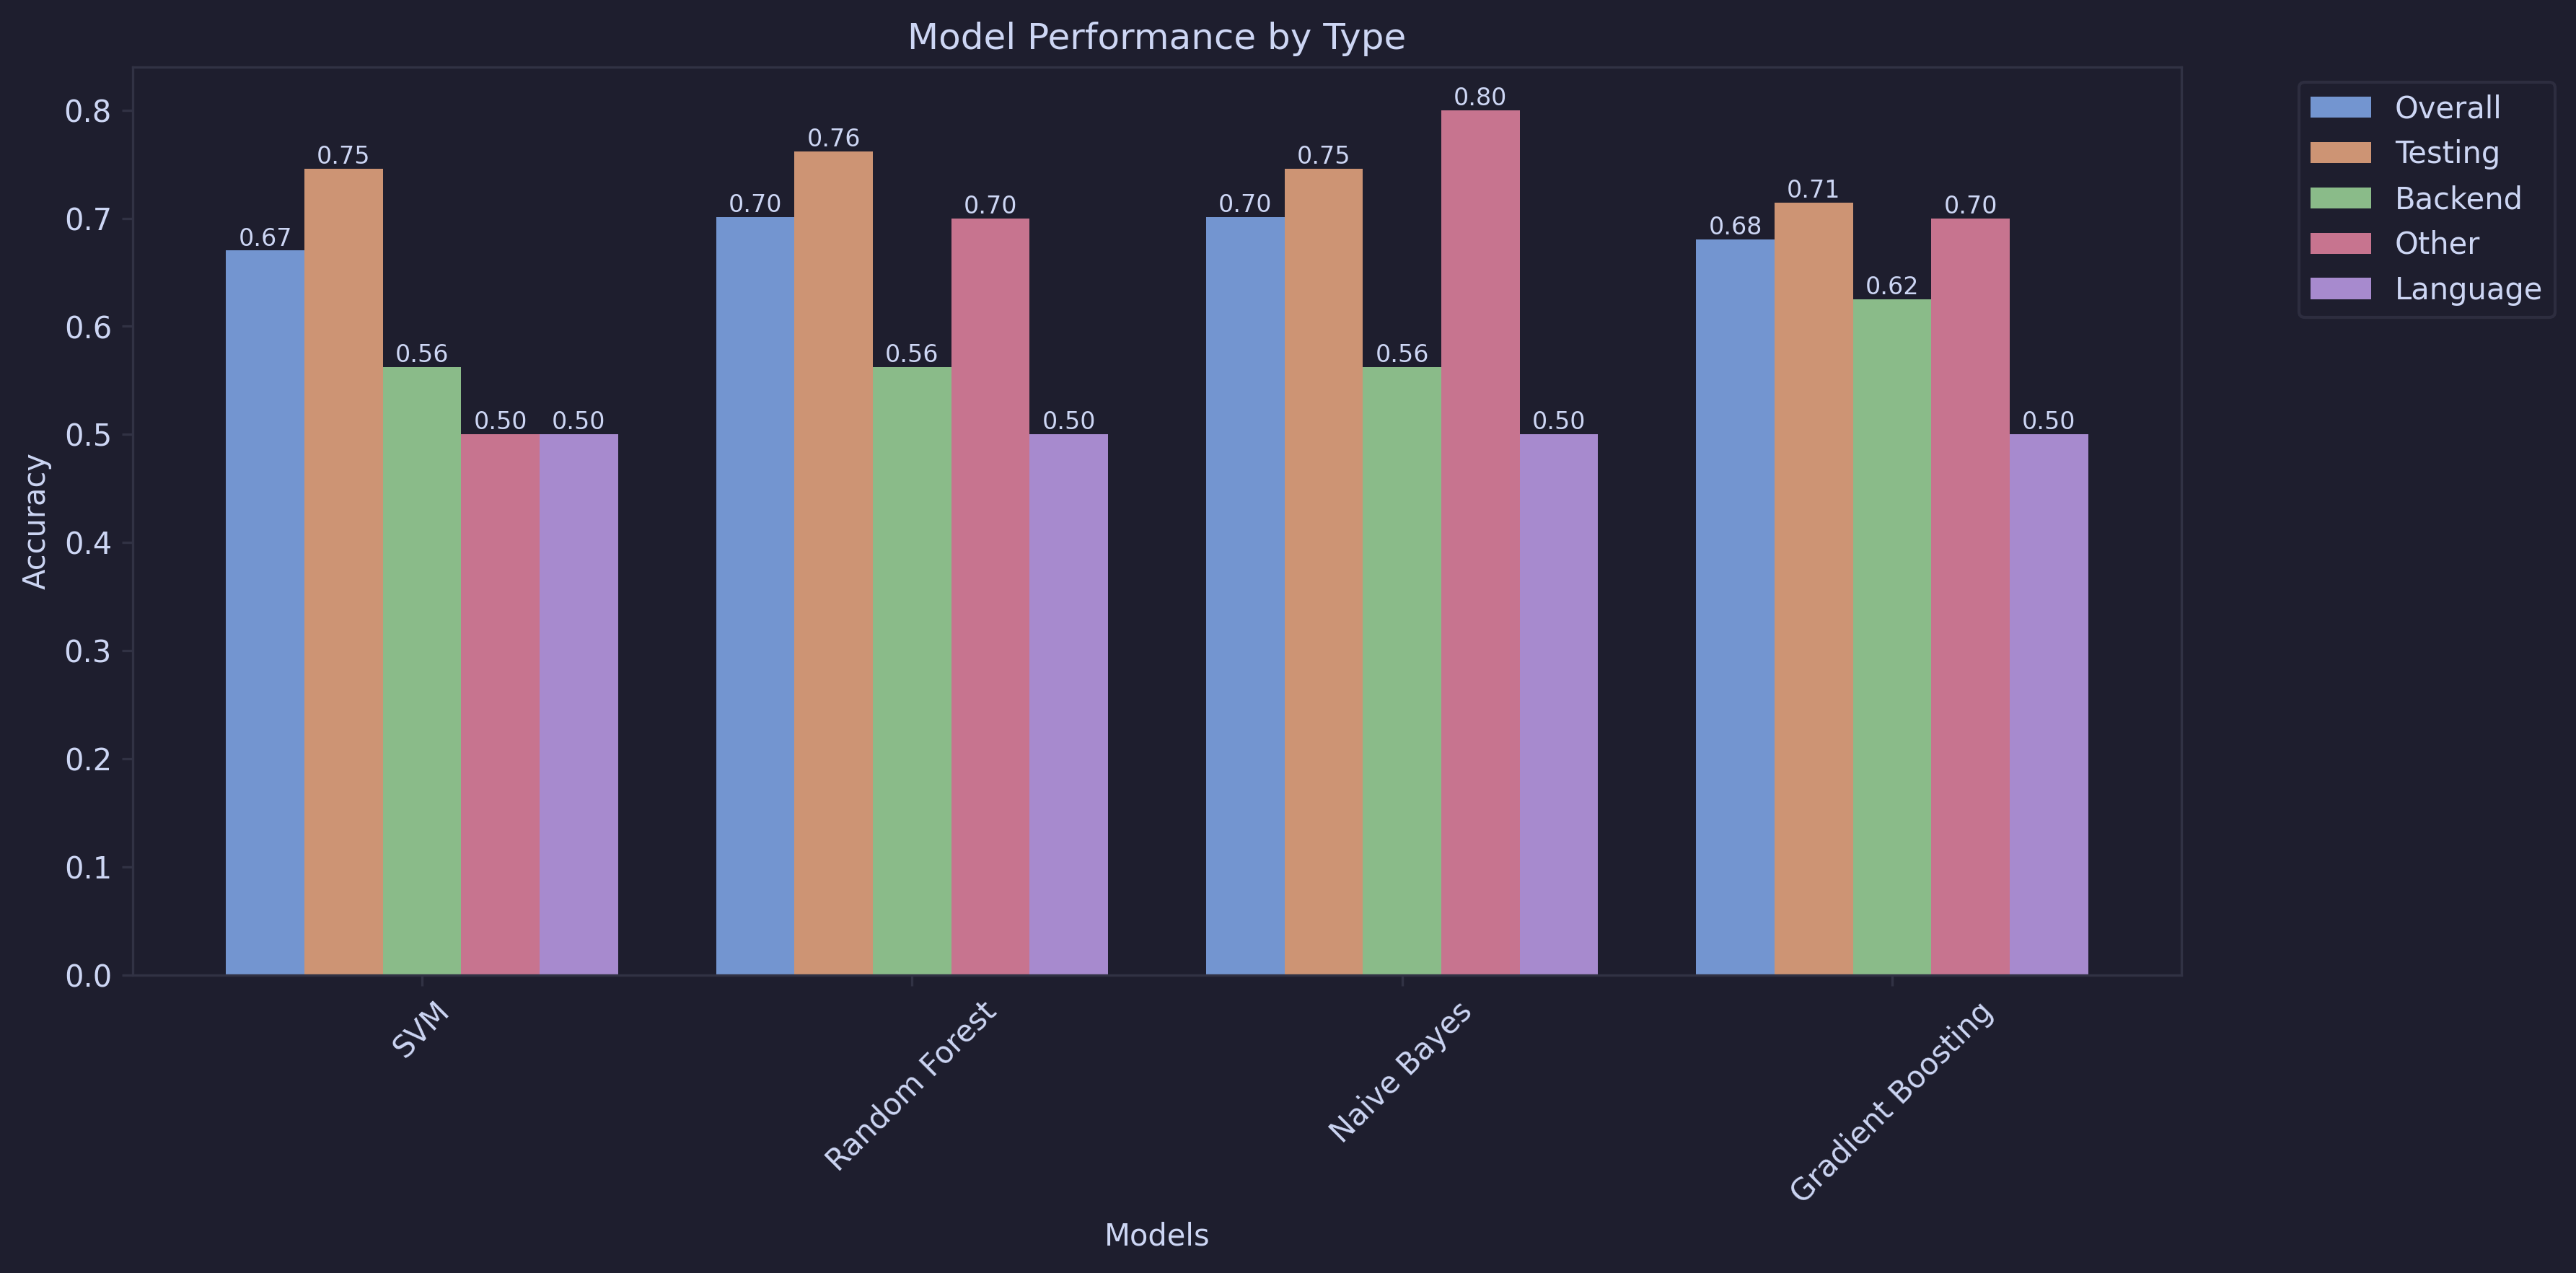
\includegraphics[width=0.9\textwidth]{best_models_type_comparison.png}
    \caption{Απόδοση μοντέλων ανά τύπο θέματος}
  \end{center}
  \label{fig:TypeQuery}
\end{figure}

\begin{figure}[H]
  \begin{center}
    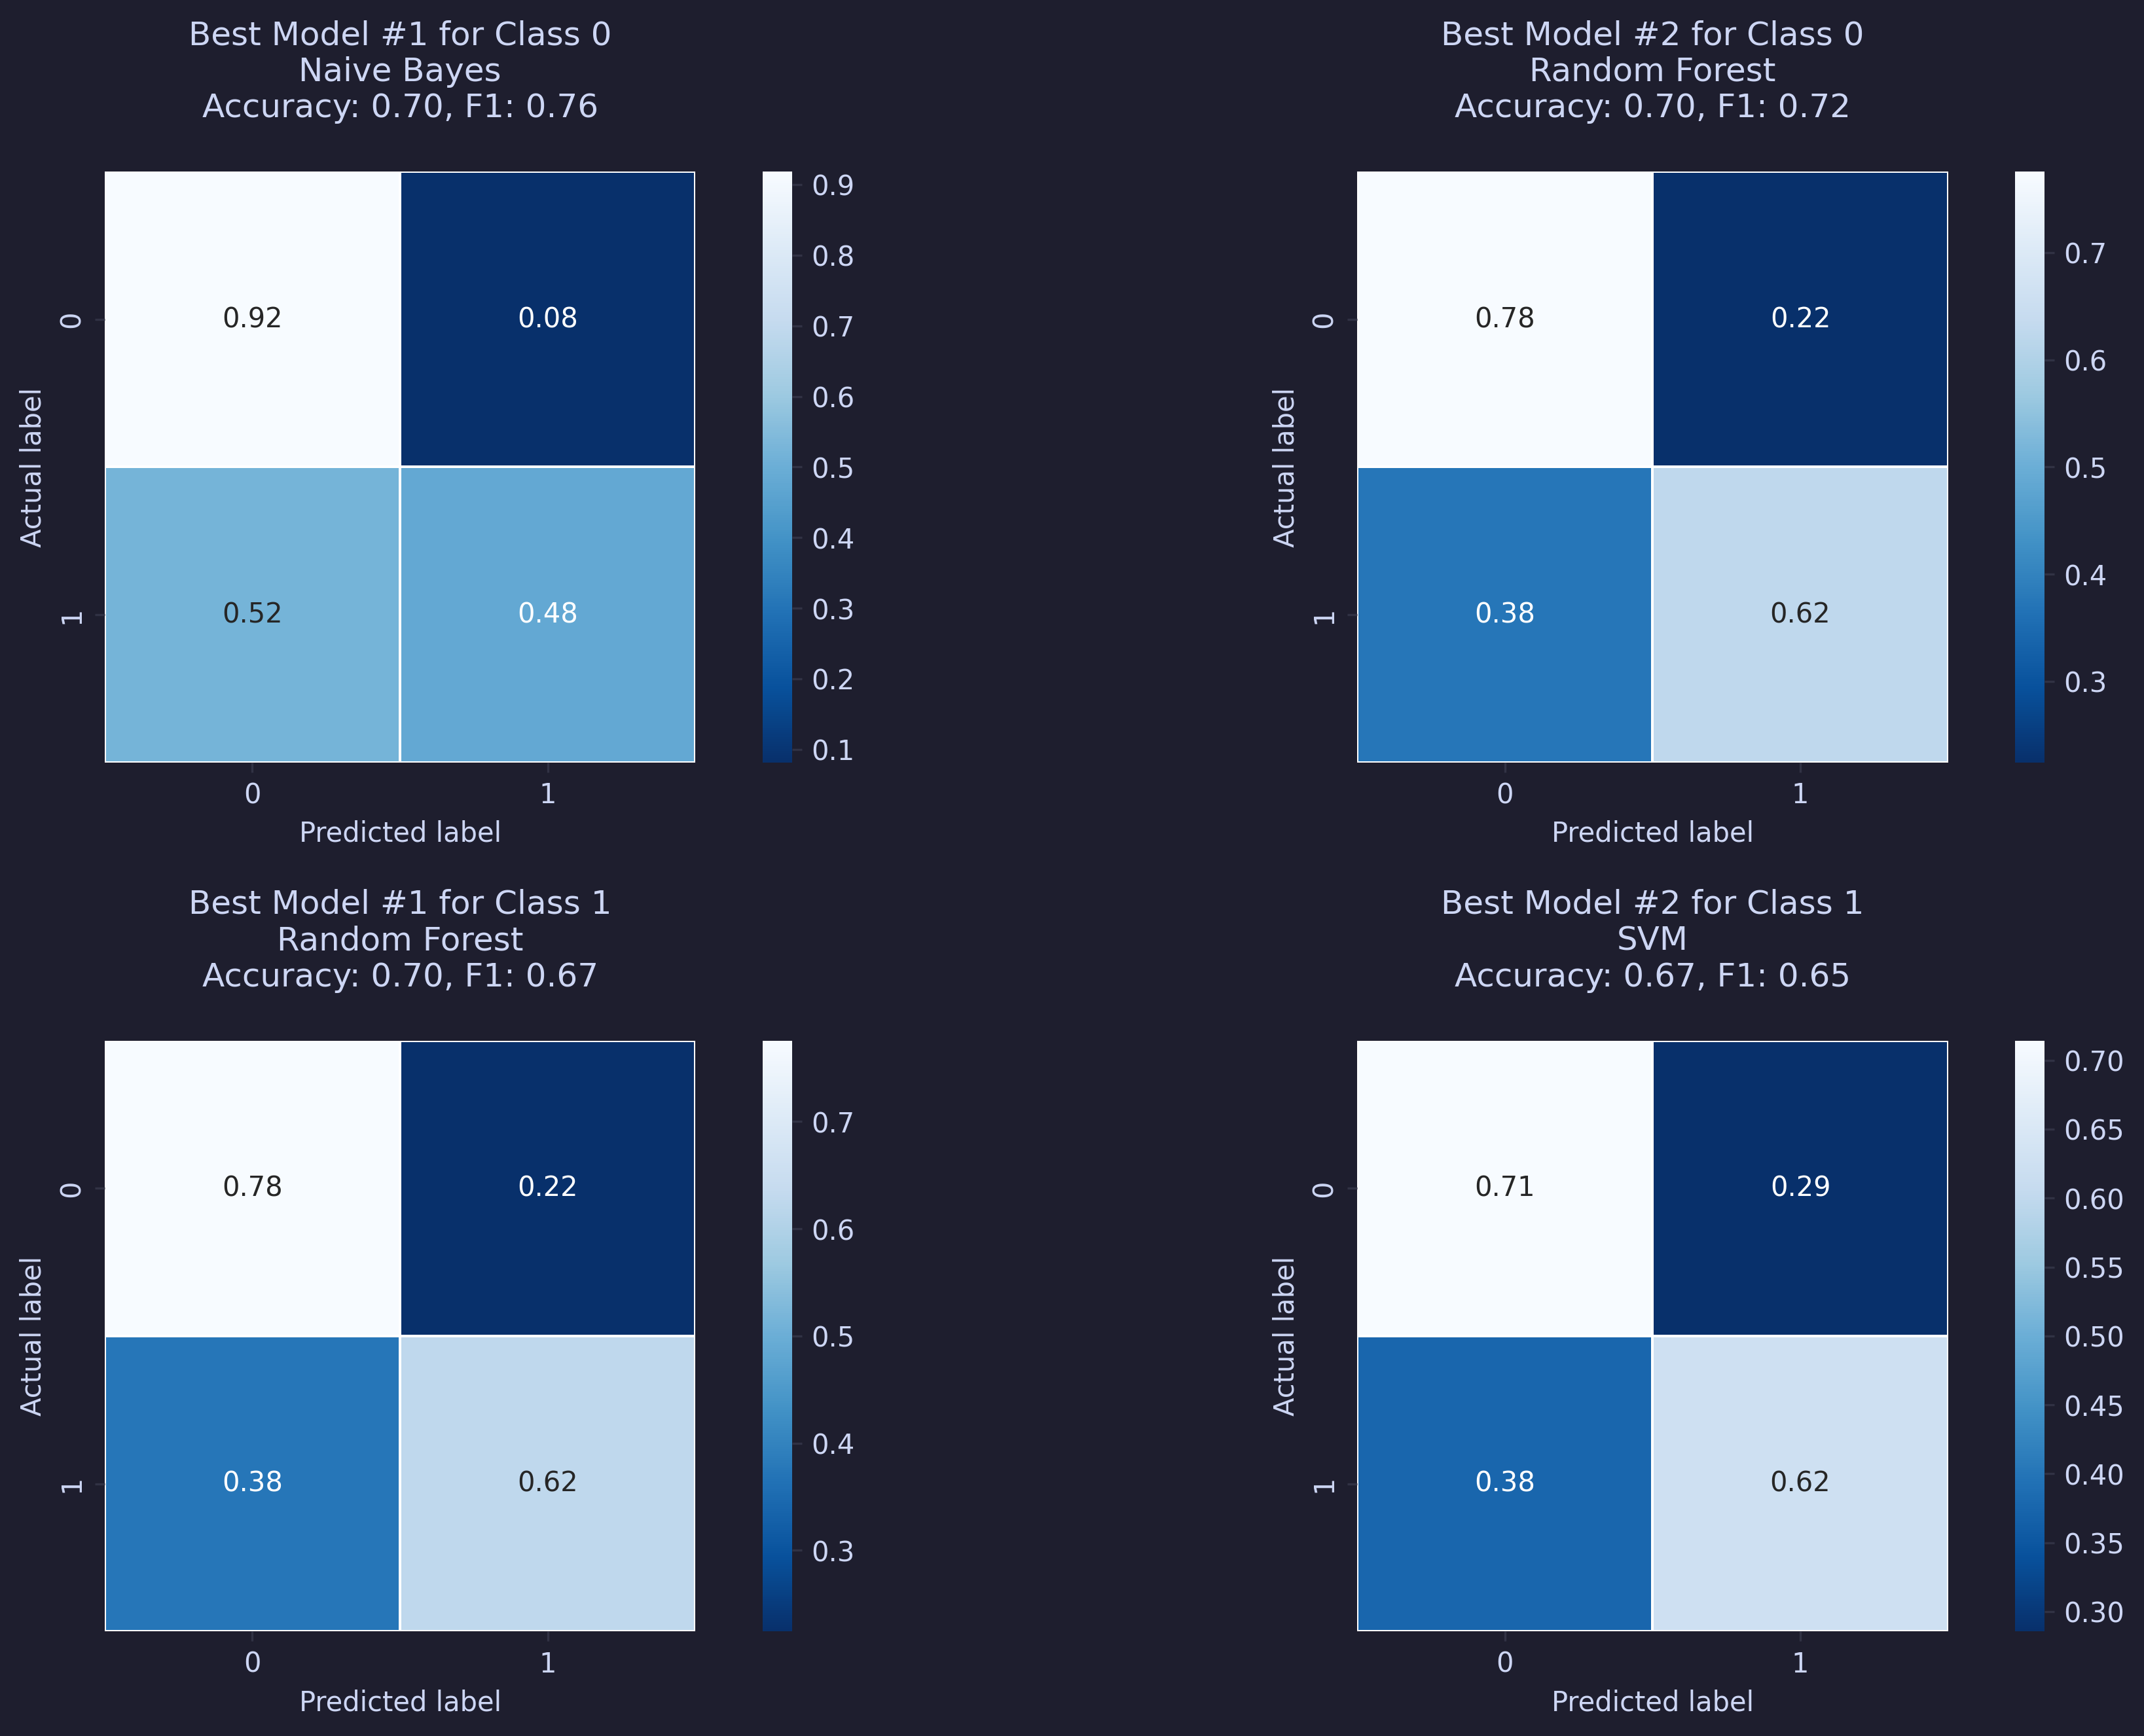
\includegraphics[width=0.9\textwidth]{best_models_per_class.png}
    \caption{Απόδοση μοντέλων ανά κλάση}
  \end{center}
  \label{fig:ClassQuery}
\end{figure}

\begin{figure}[H]
  \begin{center}
    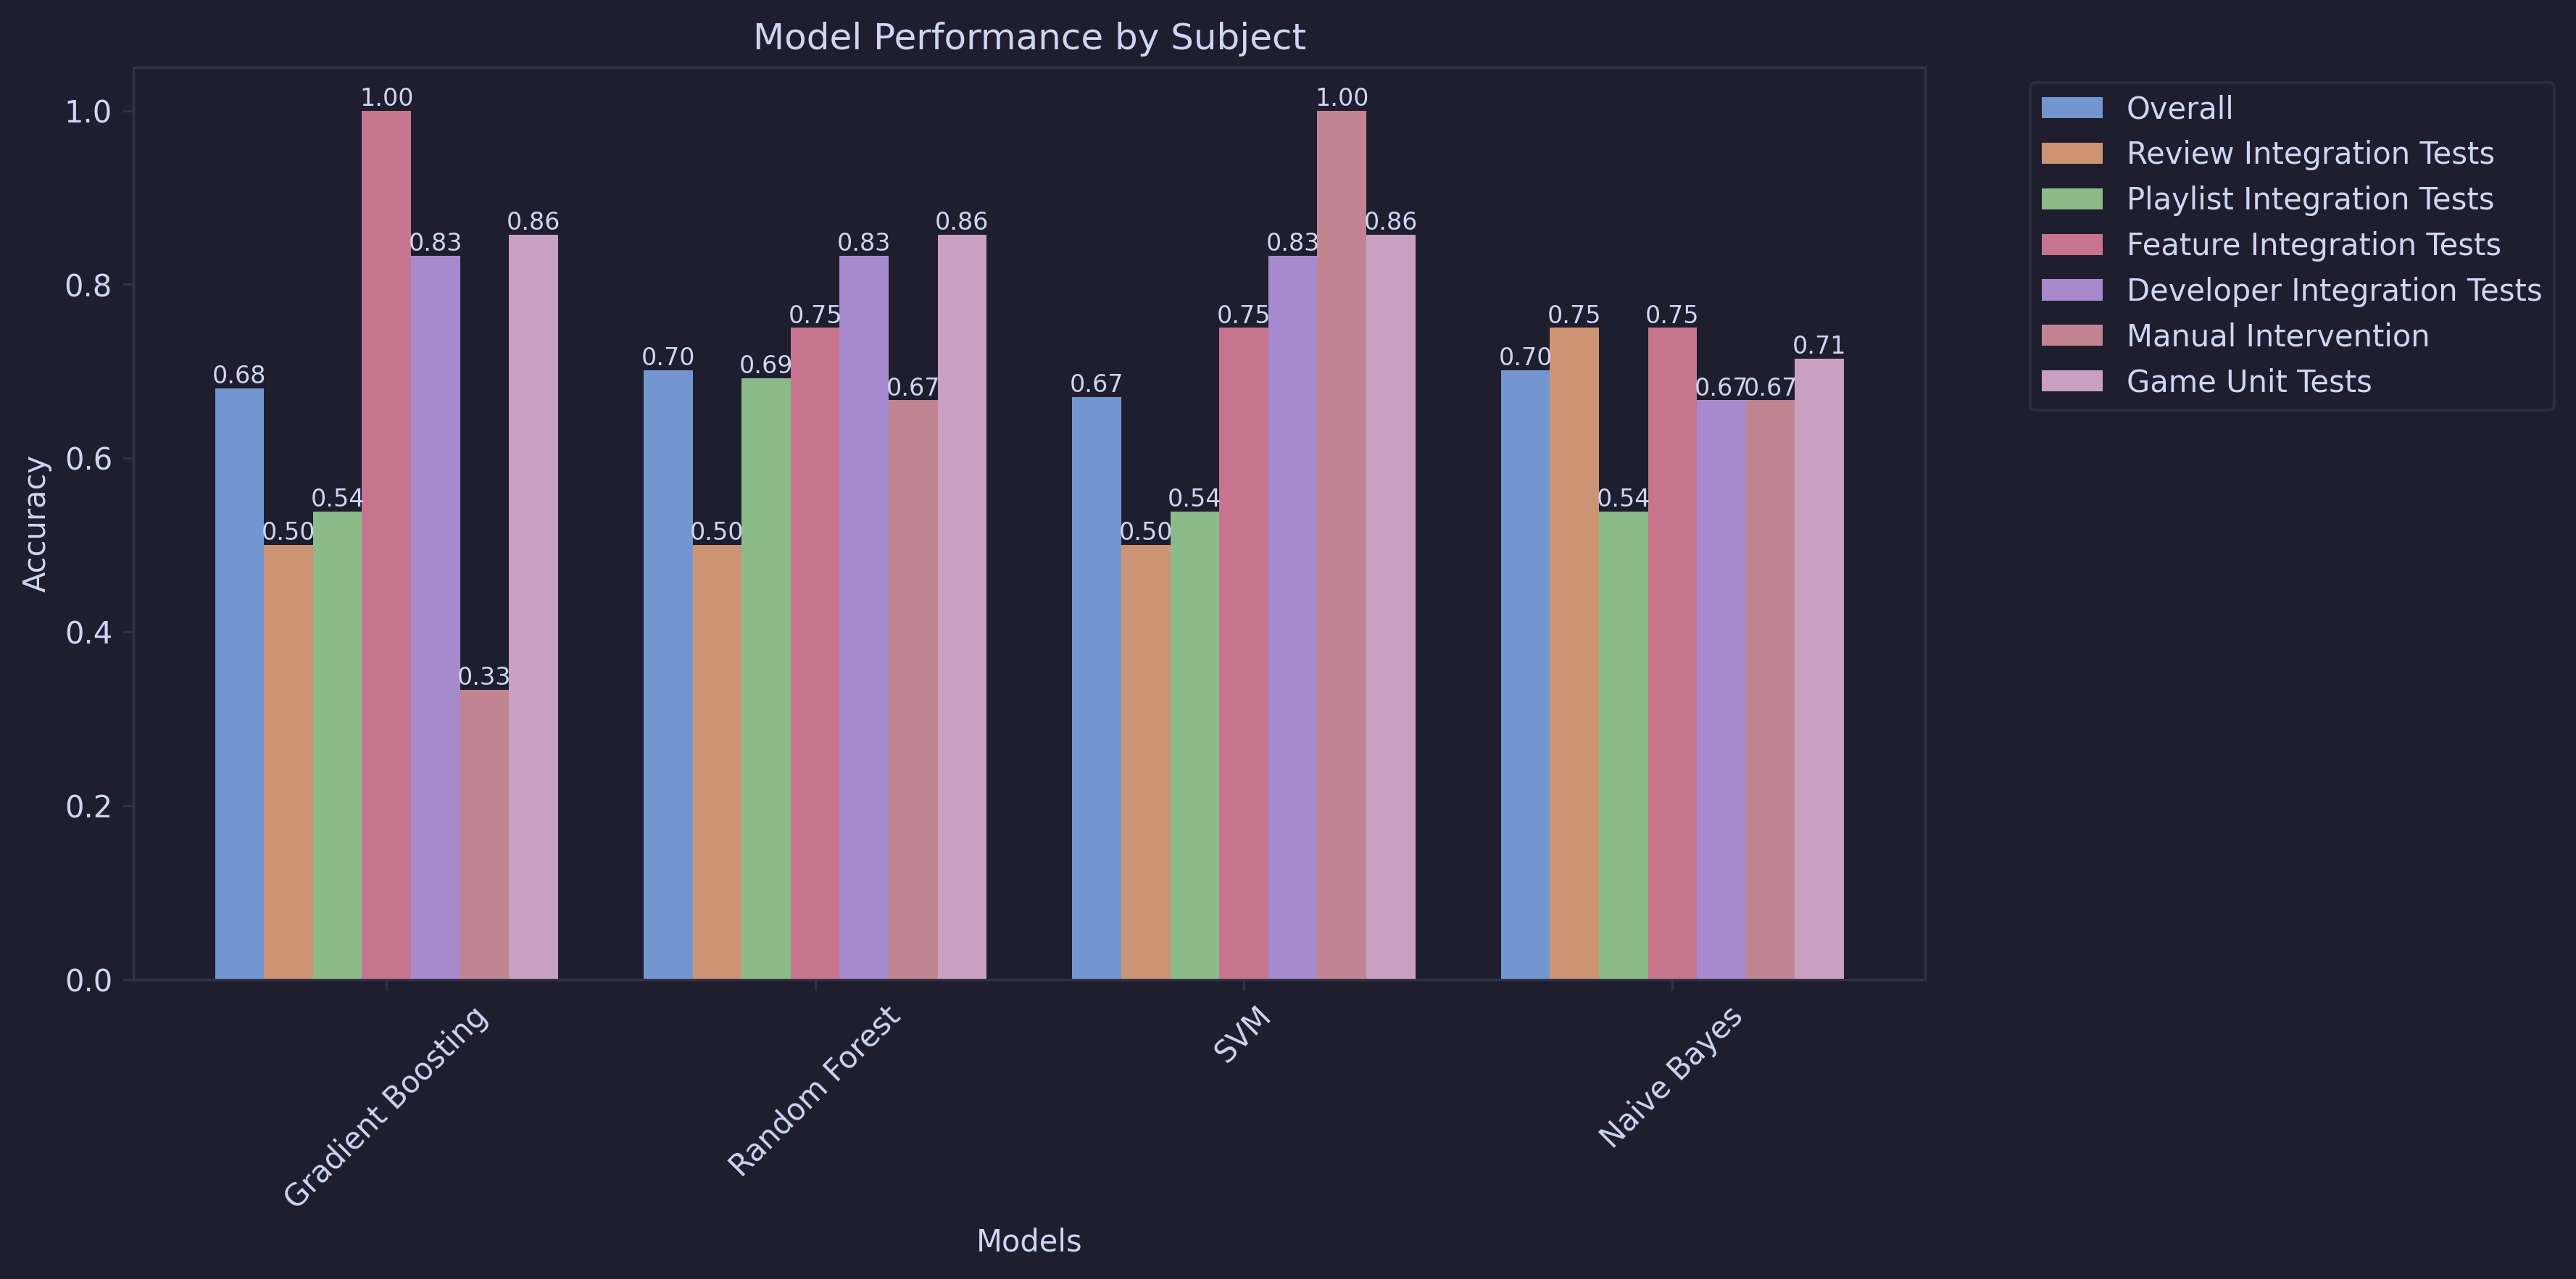
\includegraphics[width=0.9\textwidth]{best_models_subject_comparison_1.png}
    \caption{Απόδοση μοντέλων ανά θέμα, \textit{μέρος 1}}
  \end{center}
  \label{fig:Subjectres1}
\end{figure}

\begin{figure}[H]
  \begin{center}
    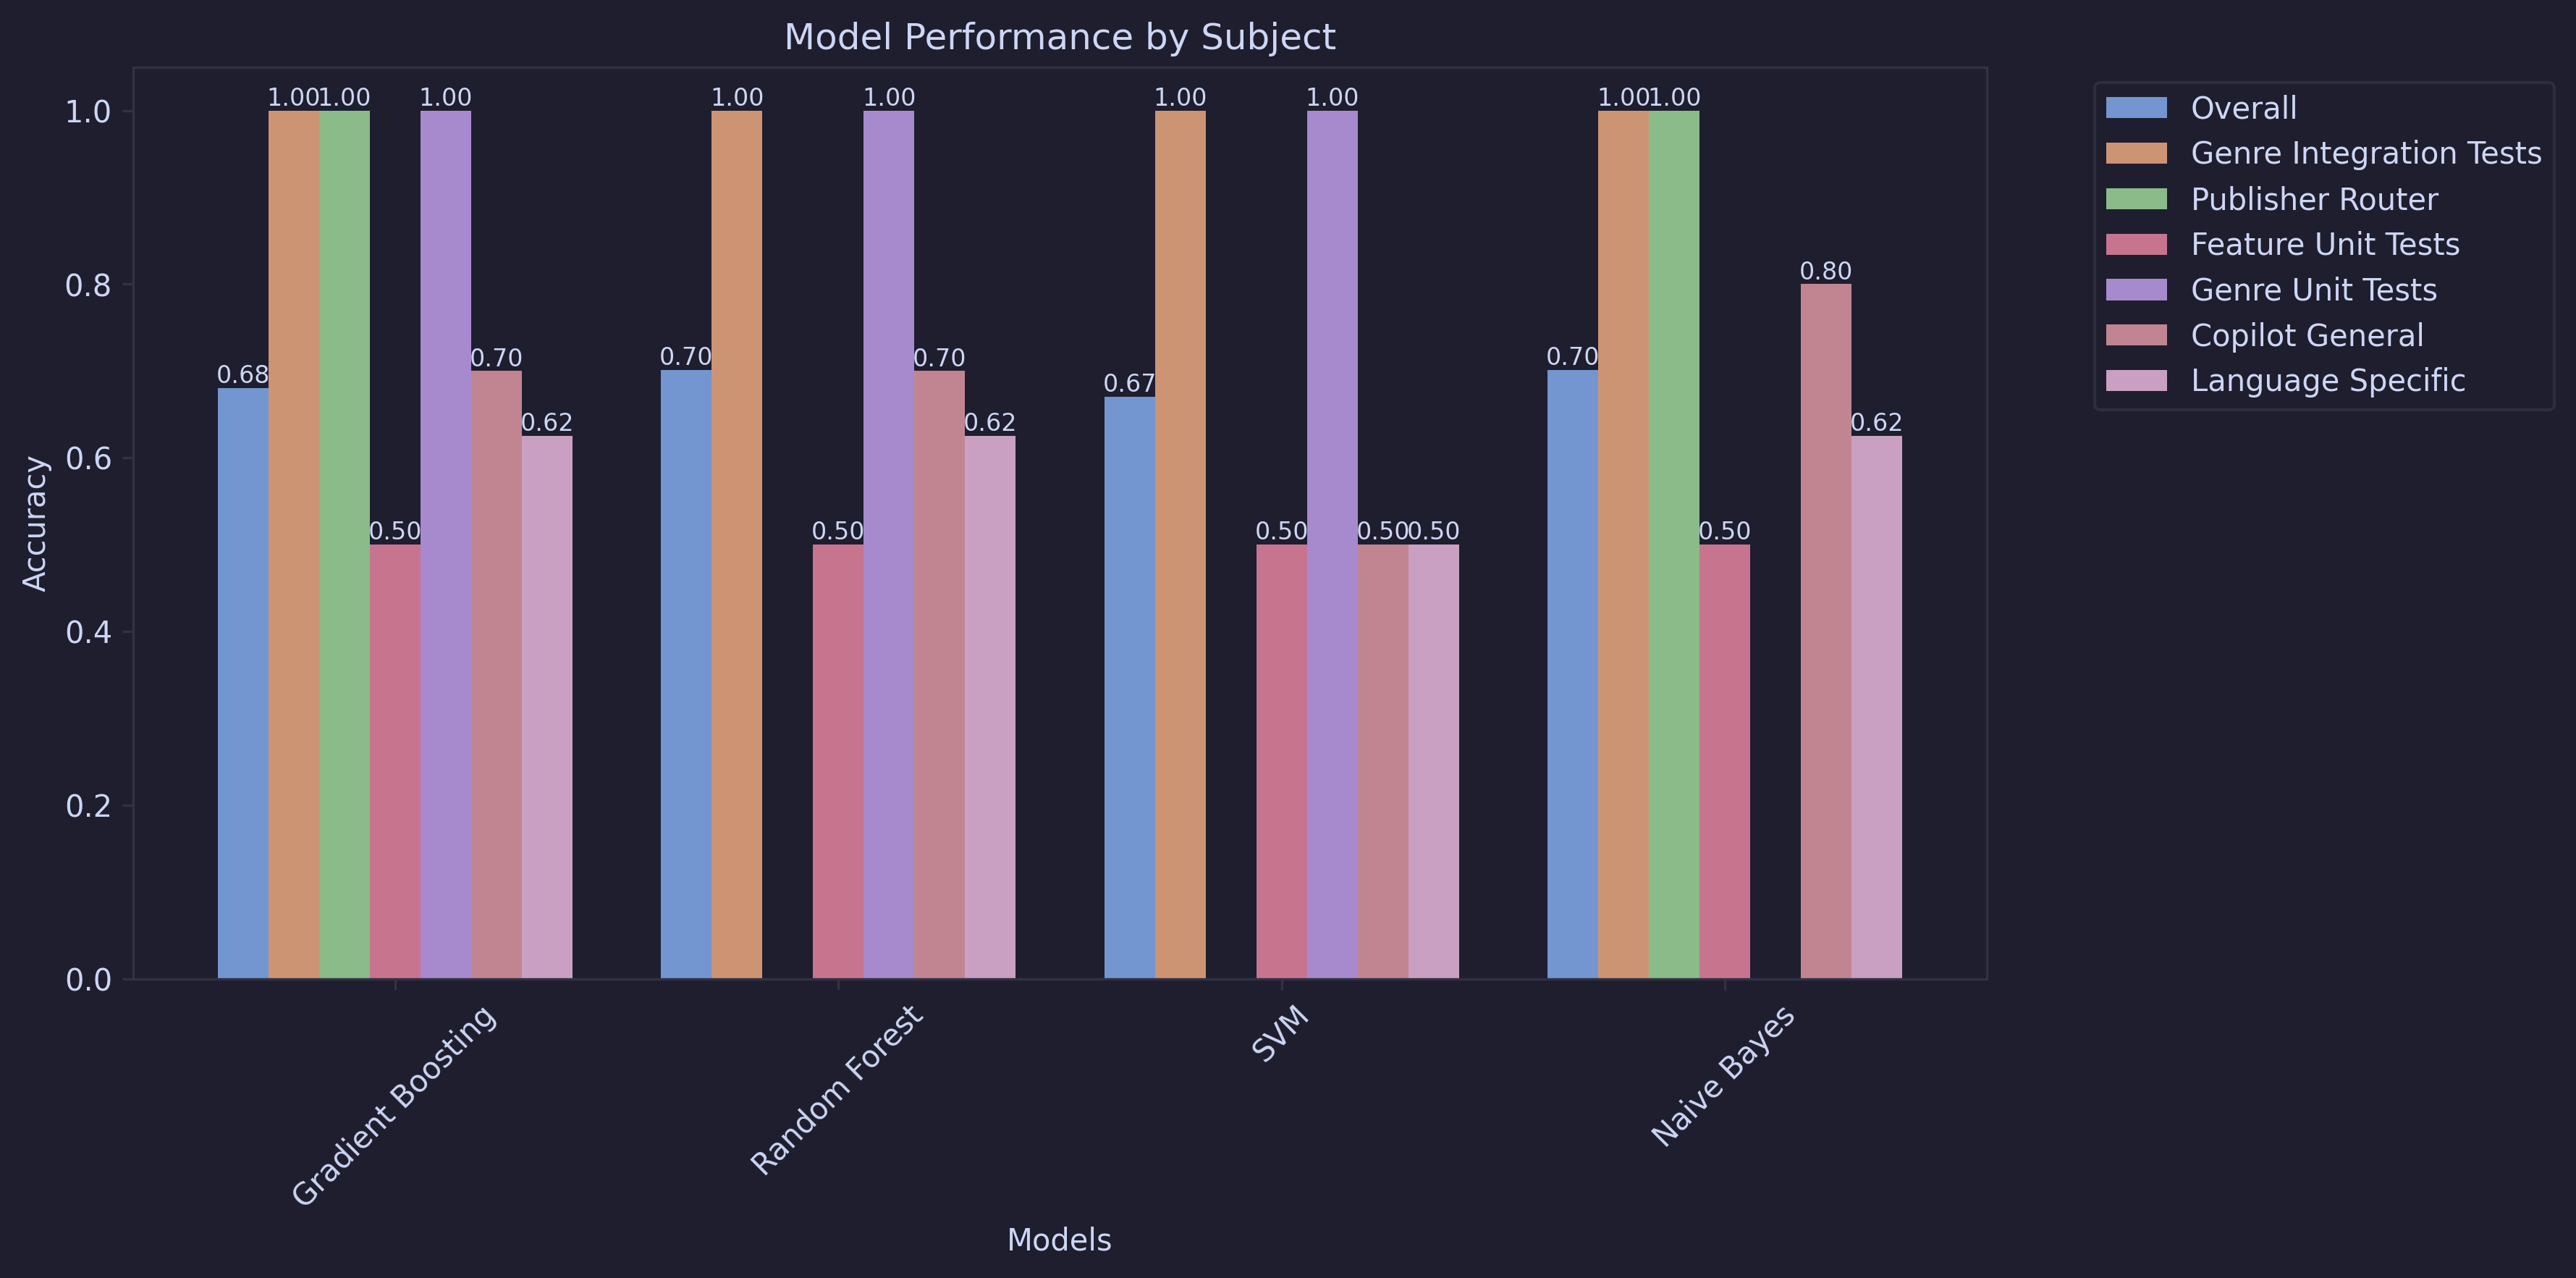
\includegraphics[width=0.9\textwidth]{best_models_subject_comparison_2.png}
    \caption{Απόδοση μοντέλων ανά θέμα, \textit{μέρος 2}}
  \end{center}
  \label{fig:Subjectres2}
\end{figure}

\begin{figure}[H]
  \begin{center}
    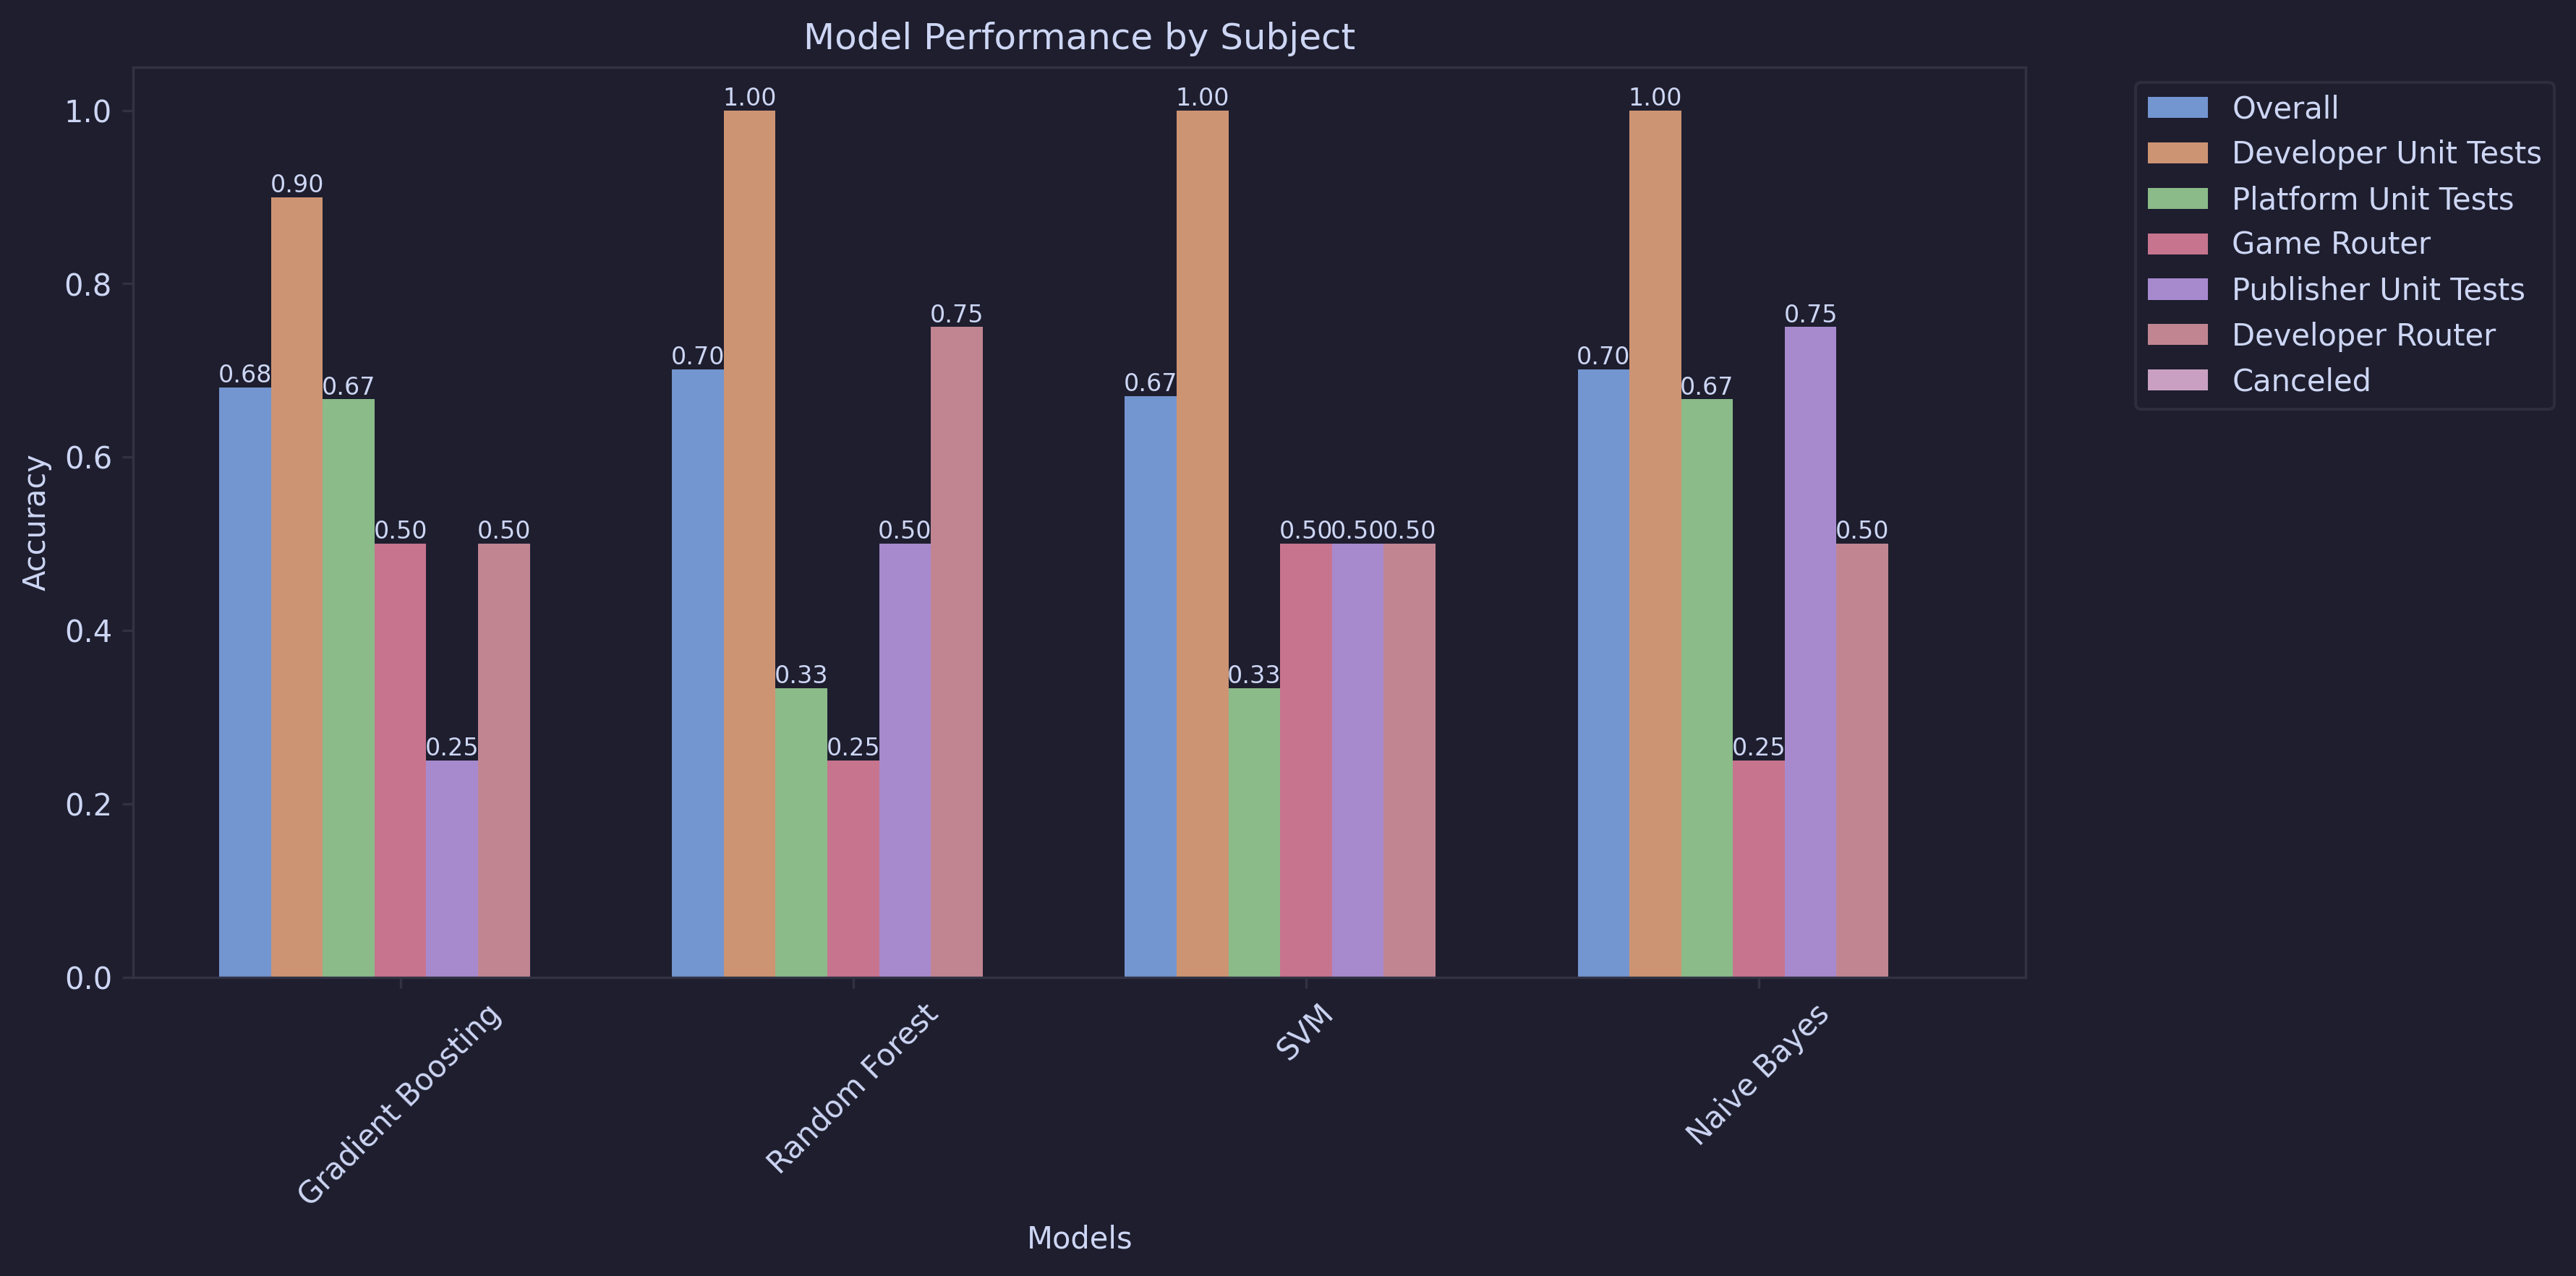
\includegraphics[width=0.9\textwidth]{best_models_subject_comparison_3.png}
    \caption{Απόδοση μοντέλων ανά θέμα, \textit{μέρος 3}}
  \end{center}
  \label{fig:Subjectres3}
\end{figure}

\begin{figure}[H]
  \begin{center}
    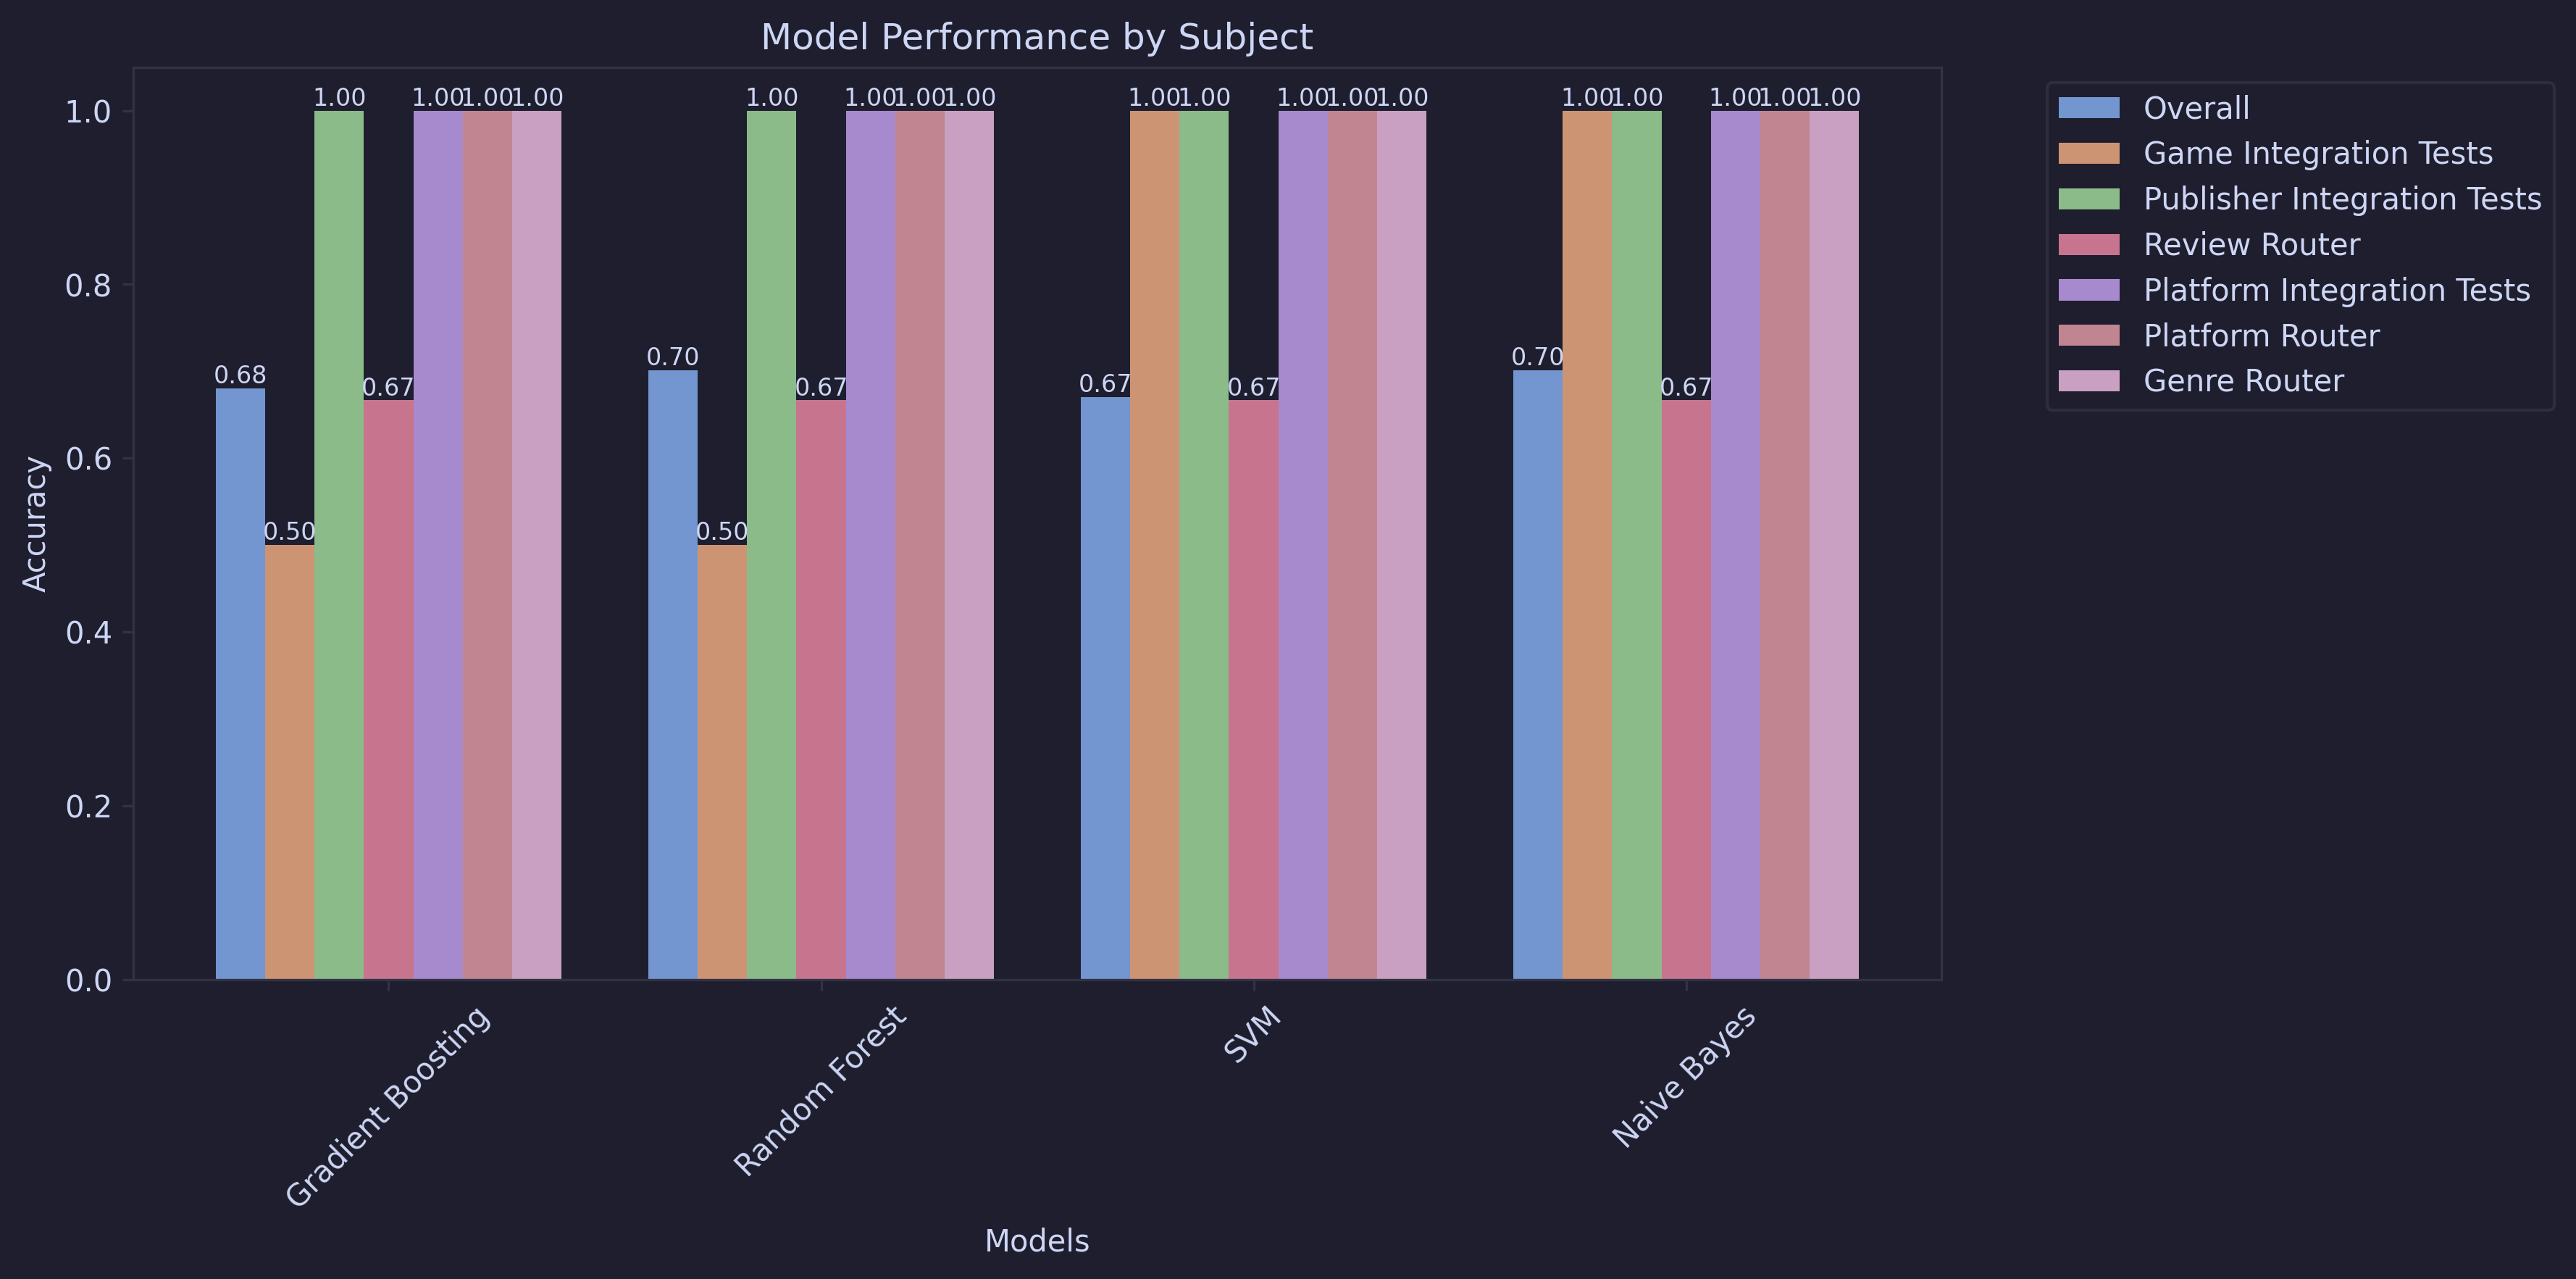
\includegraphics[width=0.9\textwidth]{best_models_subject_comparison_4.png}
    \caption{Απόδοση μοντέλων ανά θέμα, \textit{μέρος 4}}
  \end{center}
  \label{fig:Subjectres3}
\end{figure}

Το ποσοστό απόδοσης θα μπορούσε να αυξηθεί περαιτέρω με την εφαρμογή
περίσσοτερων
τεχνικών προεπεξεργασίας, όπως η εξισορρόπηση των κλάσεων, η επιλογή
χαρακτηριστικών και η βελτιστοποίηση των υπερπαραμέτρων. Επιπλέον, η
επέκταση του συνόλου δεδομένων με περισσότερες αξιολογήσεις θα μπορούσε
να βελτιώσει την απόδοση των μοντέλων.

\subsection{Συλλογή δεδομένων για περαιτέρω ανάπτυξη}
To βασικό πρόβλημα για την βελτιστοποίηση μέσω επέκτασης του συνόλου
δεδομένων αποτελεί το ηθικό δίλημμα της
συλλογής δεδομένων. Οι εταιρείες υπέυθυνες για την ανάπτυξη των
Γλωσσικών Μοντέλων, έχουν την δυνατότητα συλλογής δεδομένων των
χρηστών τους. Στην περίπτωση του \tl{GitHub Copilot}, η συλλογή
δεδομένων του χρήστη είναι ενεργή από προεπιλογή και ο χρήστης μπορεί
να ελέγξει συγκεκριμένες μόνο παραμέτρους προκειμένου να προστατέψει
τα δεδομένα του. \cite{ghcpdatacollection}. Το ίδιο ισχύει και για
την περίπτωση του \tl{ChatGPT} \cite{openaidatacollection}.

Η διεπαφή συνομιλίας του \tl{ChatGPT} και του \tl{GitHub Copilot}, έχει δύο εικονίδια-κουμπιά
για την θετική ή αρνητική αξιολόγηση της απάντησης αντίστοιχα. Τα δεδομένα αυτά αποστέλλονται αυτόματα στις
εταιρείες ανάπτυξης των μοντέλων, με σκοπό να χρησιμοποιηθούν για την συνεχόμενη ανάπτυξη των μοντέλων.

Tα δεδομένα χρηστών είναι ένα από τα πολυτιμότερα ψηφιακά αγαθά για
τις εταιρείες που αναπτύσσουν Γλωσσικά Μοντέλα, καθώς αποτελούν την
πηγή της βελτιστοποίησης των μοντέλων τους. Παρόμοιο ζήτημα αποτελεί
η συλλογή πηγαίου κώδικα για την ανάπτυξη των μοντέλων από πλατφόρμες
ελέγχου εκδόσεων. Συγκεκριμένα για την περίπτωση του \tl{GitHub},
μιας πλατφόρμας που ως επί το πλείστον ειδικεύεται στην ανάπτυξη μιας
υποδομής ασφαλούς αποθήκευσης κώδικα, όταν το μοντέλο του \tl{GitHub
Copilot} εκπαιδευόταν,
οι περισσότερες άδειες ανοιχτού λογισμικού
\cite{freesoftwaredef,ossdef,debian}, δεν είχαν κατευθυντήριες
γραμμές σε ό,τι αφορούσε την χρήση του κώδικα για την εκπαίδευση
μοντέλου.

Η άδεια \textlatin{GNU General Public License (GPL)} για παράδειμα,
θεωρείται μια άδεια \textlatin{"copyleft"}, που σημαίνει ότι απαιτεί
τα παράγωγα έργα να διανέμονται υπό τους ίδιους όρους άδειας, το
οποίο σημαίνει ότι ο κώδικας παραμένει ελεύθερος και ανοιχτός.
Η \tl{GPL} λειτουργεί ως εξής: Όταν χρησιμοποιείται κώδικας με άδεια \tl{GPL} σε
ένα έργο, ολόκληρο το έργο πρέπει να διανεμηθεί υπό την ίδια άδεια.
Αυτό διασφαλίζει ότι ο κώδικας και οποιεσδήποτε τροποποιήσεις του
παραμένουν ανοιχτές και προσβάσιμες στην κοινότητα. Οι χρήστες έχουν
το δικαίωμα να τρέχουν, να μελετούν, να μοιράζονται και να
τροποποιούν το λογισμικό. Εάν διανεμηθούν τροποποιημένες εκδόσεις,
πρέπει να είναι διαθέσιμες υπό την ίδια άδεια, διατηρώντας έτσι
την ελευθερία του λογισμικού. Eπομένως, βάσει ορισμού, κώδικας
αδειοδοτημένος από την \tl{GPL}, δεν θα μπορούσε να χρησιμοποιηθεί
κατά την ανάπτυξη ενός Γλωσσικού Μοντέλου κλειστού κώδικα, κάτι που
στην περίπτωση του \tl{GitHub Copilot}, δεν ισχύει, όπως αποδείχθηκε
από την έρευνα που σύνταξε η ομάδα του ανταγωνιστικού προϊόντος
Γλωσσικού Μοντέλου \tl{Codeium} \cite{codeiumghcp,forbes2024codeium}.
Κατά την διάρκεια της έρευνας αυτής, το μοντέλο του \tl{GitHub
Copilot} φάνηκε να
αναγνωρίζει και να ολοκληρώνει μέρη από αρχεία των διάφορων
προγραμμάτων που φέρουν την \tl{GNU}, όπως το \tl{FFMPEG},
χρησιμοποιώντας τα σχόλια σαν αρχή της προτροπής, με το μοντέλο να
ακολουθεί πιστά τον πηγαίο κώδικα.

Στα πλαίσια της τεχνητής νοημοσύνης, δεν υπάρχει ακόμα συγκεκριμένος
ορισμός για την ανοιχτή και ελεύθερη τεχνητή νοημοσύνη, καθώς ακόμα ο
οργανισμός \tl{Open Source Initiave}, δεν έχει ακόμα εκδόσει επίσημο
ορισμό για την ανοιχτή τεχνητή νοημοσύνη, αφού βρίσκεται ακόμα σε
καθεστώς υποψήφιας
έκδοσης του ορισμού \tl{(Release Candidate, RC)}
\cite{OpenSourceAIDefinition}. O οργανιμός \tl{Open Source Initiave}
είναι υπεύθυνος
για την προώθηση, την εκπαίδευση και την υπεράσπιση των αρχών του
ανοιχτού λογισμικού, τη διατήρηση του Ορισμού Ανοιχτού Κώδικα και τη
δημιουργία γεφυρών μεταξύ διαφορετικών κοινοτήτων στο οικοσύστημα του
ανοιχτού κώδικα εν γένει.

Στην περίπτωση της τεχνητής νοημοσύνης, ο όρος Ανοιχτός Κώδικας δεν
αφορά αποκλειστικά τον πηγαίο κωδικά, αλλά και τα δεδομένα που
χρησιμοποιήθηκαν για την ανάπτυξη ενός μοντέλου.
Παρεθένoντας τον ορισμό της ανοικτής τεχνητής νοημοσύνης από την
υποψήφια έκδοση του \tl{Open Source Initiative}, ως εξής:

\say{Συγκεκριμένα, αυτό [οι πληροφορίες για τα δεδομένα] πρέπει να
  περιλαμβάνει: (1) μια λεπτομερή περιγραφή όλων των δεδομένων που
  χρησιμοποιούνται για την εκπαίδευση, συμπεριλαμβανομένων (εάν
  χρησιμοποιούνται) των μη κοινοποιήσιμων δεδομένων, αποκαλύπτοντας
  την προέλευση των δεδομένων, το εύρος και τα χαρακτηριστικά τους,
  πώς αποκτήθηκαν και επιλέχθηκαν τα δεδομένα, τις διαδικασίες
  επισήμανσης και τις μεθοδολογίες καθαρισμού δεδομένων· (2) μια
  λίστα όλων των δημόσια διαθέσιμων δεδομένων εκπαίδευσης και πού να
  τα αποκτήσετε· και (3) μια λίστα όλων των δεδομένων εκπαίδευσης που
  μπορούν να αποκτηθούν από τρίτους και πού να τα αποκτήσετε,
  συμπεριλαμβανομένων αυτών με χρέωση.}

Ιδιαίτερο ενδιαφέρον παρουσιάζει η περίπτωση του μοντέλου \tl{Llama} της
εταιρείας \tl{Meta} (παλαιότερα \tl{Facebook})\cite{llama}.
Το συγκεκριμένο μοντέλο, παρουσιάζεται από την εταιρεία \tl{Meta} ως
ένα μοντέλο ανοιχτού κώδικα, καθώς ο πηγαίος κώδικας είναι δημόσιος
στην πλατφόρμα του \tl{GitHub}.
Ωστόσο, τόσο η συλλογή δεδομένων, όσο και η επιλογή της άδειας του
κώδικα αποτελούν πηγή συζητήσεων σχετικά με την εγκυρότητά τους.
Αρχικά, η πηγή από την οποία συλλέχθηκαν τα δεδομένα, δεν είναι
γνωστή. \cite{llama3}
Η άδεια του λογισμικού όμως, είναι το μεγαλύτερο ζήτημα. Το \tl{Llama
3.2}, είναι αδειοδοτημένο από την ομώνυμη άδεια, η οποία δεν είναι
επίσημα υιοθετημένη από το \tl{Open Source Initiave}. Αυτό οφείλεται
σε ορισμένους κανόνες χρήσης του λογισμικού \cite{llamalicense}:

\begin{itemize}
  \item \say{Δεν θα χρησιμοποιήσετε τα Υλικά \tl{Llama} ή οποιαδήποτε
      έξοδο ή αποτελέσματα των Υλικών \tl{Llama} για τη βελτίωση
      οποιουδήποτε άλλου μεγάλου γλωσσικού μοντέλου (εξαιρουμένου του
    \tl{Llama} 2 ή παράγωγων έργων αυτού).} (To \tl{Llama 3.2}
    υπόκειται στα παράγωγα έργα του \tl{Llama 2})
  \item \say{Πρόσθετοι Εμπορικοί Όροι. Εάν, κατά την ημερομηνία
      κυκλοφορίας της έκδοσης \tl{Llama} 2, οι μηνιαίοι ενεργοί χρήστες
      των προϊόντων ή υπηρεσιών που διατίθενται από ή για τον Αδειούχο,
      ή τις συνδεδεμένες εταιρείες του Αδειούχου, υπερβαίνουν τους 700
      εκατομμύρια μηνιαίους ενεργούς χρήστες κατά τον προηγούμενο
      ημερολογιακό μήνα, πρέπει να ζητήσετε άδεια από τη \tl{Meta}, την
      οποία η \tl{Meta} μπορεί να σας παραχωρήσει κατά την απόλυτη
      διακριτική της ευχέρεια και δεν έχετε εξουσιοδότηση να ασκήσετε
      οποιοδήποτε από τα δικαιώματα βάσει αυτής της Συμφωνίας εκτός εάν
    ή μέχρις ότου η \tl{Meta} σας παραχωρήσει ρητά τέτοια δικαιώματα.}
\end{itemize}

Οι παραπάνω όροι έρχονται σε έντονη αντίθεση με τον ορισμό του
λογισμικού ανοιχτού κώδικα, περιορίζοντας τη χρήση του κώδικα με
τρόπους που δεν διευκολύνουν την ανοιχτή και ελεύθερη διανομή λογισμικού.

Η εκπαίδευση ενός μοντέλου μηχανικής μάθησης για την πρόβλεψη της
απάντησης ενός Γλωσσικού Μοντέλου μέσω της προτροπής, πρέπει να
αποκτήσει τα απαραίτητα δεδομένα μέσω απόφασης χρηστών, το οποίο
ξεπερνά το πλαίσιο αυτής της διατριβής.

